% Options for packages loaded elsewhere
\PassOptionsToPackage{unicode}{hyperref}
\PassOptionsToPackage{hyphens}{url}
%
\documentclass[
  english,
  jou,floatsintext]{apa6}
\usepackage{lmodern}
\usepackage{amssymb,amsmath}
\usepackage{ifxetex,ifluatex}
\ifnum 0\ifxetex 1\fi\ifluatex 1\fi=0 % if pdftex
  \usepackage[T1]{fontenc}
  \usepackage[utf8]{inputenc}
  \usepackage{textcomp} % provide euro and other symbols
\else % if luatex or xetex
  \usepackage{unicode-math}
  \defaultfontfeatures{Scale=MatchLowercase}
  \defaultfontfeatures[\rmfamily]{Ligatures=TeX,Scale=1}
\fi
% Use upquote if available, for straight quotes in verbatim environments
\IfFileExists{upquote.sty}{\usepackage{upquote}}{}
\IfFileExists{microtype.sty}{% use microtype if available
  \usepackage[]{microtype}
  \UseMicrotypeSet[protrusion]{basicmath} % disable protrusion for tt fonts
}{}
\makeatletter
\@ifundefined{KOMAClassName}{% if non-KOMA class
  \IfFileExists{parskip.sty}{%
    \usepackage{parskip}
  }{% else
    \setlength{\parindent}{0pt}
    \setlength{\parskip}{6pt plus 2pt minus 1pt}}
}{% if KOMA class
  \KOMAoptions{parskip=half}}
\makeatother
\usepackage{xcolor}
\IfFileExists{xurl.sty}{\usepackage{xurl}}{} % add URL line breaks if available
\IfFileExists{bookmark.sty}{\usepackage{bookmark}}{\usepackage{hyperref}}
\hypersetup{
  pdftitle={Videogaming effects on mental health outcomes during three COVID-19 national lockdowns},
  pdfauthor={Sophie Hodgetts1, Glenn Patrick Williams1, Jon Rees1, \& Joe Butler1},
  pdflang={en-EN},
  pdfkeywords={keywords},
  hidelinks,
  pdfcreator={LaTeX via pandoc}}
\urlstyle{same} % disable monospaced font for URLs
\usepackage{graphicx,grffile}
\makeatletter
\def\maxwidth{\ifdim\Gin@nat@width>\linewidth\linewidth\else\Gin@nat@width\fi}
\def\maxheight{\ifdim\Gin@nat@height>\textheight\textheight\else\Gin@nat@height\fi}
\makeatother
% Scale images if necessary, so that they will not overflow the page
% margins by default, and it is still possible to overwrite the defaults
% using explicit options in \includegraphics[width, height, ...]{}
\setkeys{Gin}{width=\maxwidth,height=\maxheight,keepaspectratio}
% Set default figure placement to htbp
\makeatletter
\def\fps@figure{htbp}
\makeatother
\setlength{\emergencystretch}{3em} % prevent overfull lines
\providecommand{\tightlist}{%
  \setlength{\itemsep}{0pt}\setlength{\parskip}{0pt}}
\setcounter{secnumdepth}{-\maxdimen} % remove section numbering
% Make \paragraph and \subparagraph free-standing
\ifx\paragraph\undefined\else
  \let\oldparagraph\paragraph
  \renewcommand{\paragraph}[1]{\oldparagraph{#1}\mbox{}}
\fi
\ifx\subparagraph\undefined\else
  \let\oldsubparagraph\subparagraph
  \renewcommand{\subparagraph}[1]{\oldsubparagraph{#1}\mbox{}}
\fi
% Manuscript styling
\usepackage{upgreek}
\captionsetup{font=singlespacing,justification=justified}

% Table formatting
\usepackage{longtable}
\usepackage{lscape}
% \usepackage[counterclockwise]{rotating}   % Landscape page setup for large tables
\usepackage{multirow}		% Table styling
\usepackage{tabularx}		% Control Column width
\usepackage[flushleft]{threeparttable}	% Allows for three part tables with a specified notes section
\usepackage{threeparttablex}            % Lets threeparttable work with longtable

% Create new environments so endfloat can handle them
% \newenvironment{ltable}
%   {\begin{landscape}\begin{center}\begin{threeparttable}}
%   {\end{threeparttable}\end{center}\end{landscape}}
\newenvironment{lltable}{\begin{landscape}\begin{center}\begin{ThreePartTable}}{\end{ThreePartTable}\end{center}\end{landscape}}

% Enables adjusting longtable caption width to table width
% Solution found at http://golatex.de/longtable-mit-caption-so-breit-wie-die-tabelle-t15767.html
\makeatletter
\newcommand\LastLTentrywidth{1em}
\newlength\longtablewidth
\setlength{\longtablewidth}{1in}
\newcommand{\getlongtablewidth}{\begingroup \ifcsname LT@\roman{LT@tables}\endcsname \global\longtablewidth=0pt \renewcommand{\LT@entry}[2]{\global\advance\longtablewidth by ##2\relax\gdef\LastLTentrywidth{##2}}\@nameuse{LT@\roman{LT@tables}} \fi \endgroup}

% \setlength{\parindent}{0.5in}
% \setlength{\parskip}{0pt plus 0pt minus 0pt}

% \usepackage{etoolbox}
\makeatletter
\patchcmd{\HyOrg@maketitle}
  {\section{\normalfont\normalsize\abstractname}}
  {\section*{\normalfont\normalsize\abstractname}}
  {}{\typeout{Failed to patch abstract.}}
\patchcmd{\HyOrg@maketitle}
  {\section{\protect\normalfont{\@title}}}
  {\section*{\protect\normalfont{\@title}}}
  {}{\typeout{Failed to patch title.}}
\makeatother
\shorttitle{Covid Gaming}
\keywords{keywords\newline\indent Word count: X}
\usepackage{dblfloatfix}


\usepackage{lineno}

\linenumbers
\usepackage{csquotes}
\usepackage{tipa}
\usepackage{float}
\usepackage{hyperref}
\usepackage{makecell}
\ifxetex
  % Load polyglossia as late as possible: uses bidi with RTL langages (e.g. Hebrew, Arabic)
  \usepackage{polyglossia}
  \setmainlanguage[]{english}
\else
  \usepackage[shorthands=off,main=english]{babel}
\fi

\title{Videogaming effects on mental health outcomes during three COVID-19 national lockdowns}
\author{Sophie Hodgetts\textsuperscript{1}, Glenn Patrick Williams\textsuperscript{1}, Jon Rees\textsuperscript{1}, \& Joe Butler\textsuperscript{1}}
\date{}


\authornote{

School of Psychology, Faculty of Health Sciences and Wellbeing, University of Sunderland, Sunderland, SR1 3SD, England, UK.

Pre-registration, data and code, and pre-print are available at\ldots{}

This preprint has not been peer reviewed.

The authors made the following contributions. Sophie Hodgetts: Conceptualization, Investigation, Data curation, Methodology, Project Administration, Resources, Writing - Original Draft Preparation, Writing - Review \& Editing; Glenn Patrick Williams: Writing - Review \& Editing, Data Curation, Methodology, Formal Analysis, Visualization; Jon Rees: Methodology, Formal Analysis, Writing - Review \& Editing; Joe Butler: Conceptualization, Investigation, Methodology, Writing - Review \& Editing.

Correspondence concerning this article should be addressed to Sophie Hodgetts, Postal address. E-mail: \href{mailto:sophie.hodgetts@sunderland.ac.uk}{\nolinkurl{sophie.hodgetts@sunderland.ac.uk}}

}

\affiliation{\vspace{0.5cm}\textsuperscript{1} University of Sunderland}

\abstract{
Abstract goes here.
}



\begin{document}
\maketitle

\hypertarget{introduction}{%
\section{Introduction}\label{introduction}}

Intro here.

\hypertarget{methods}{%
\section{Methods}\label{methods}}

\hypertarget{participants}{%
\subsection{Participants}\label{participants}}

Five hundred and seventy-one participants were recruited to take part in this study online via Qualtrics. Of which 344 provided full informed consent. One hundred and fifty participants were excluded from this sample due to having completed less than 90\% of the questionnaire, providing invalid employment details (i.e.~stating they were both employed and unemployed) or for reporting having played no games before or during lockdown. A further 39 participants were removed from the analysis due to having more than 20\% of trials with missing data and/or having reported hours played more than 3 MAD above the median hours played in games in an average week (i.e.~around 150 hours). After all exclusions we analysed data from 155 participants (age \emph{M} = 32.58, \emph{SD} = 8.94, Range = 19 - 72). On average participants took 23.84 minutes to complete the task (\emph{SD} = 58.43).

The below graph shows the number of participants in a given employment situation during lockdown.

\begin{figure*}[!htbp]

{\centering 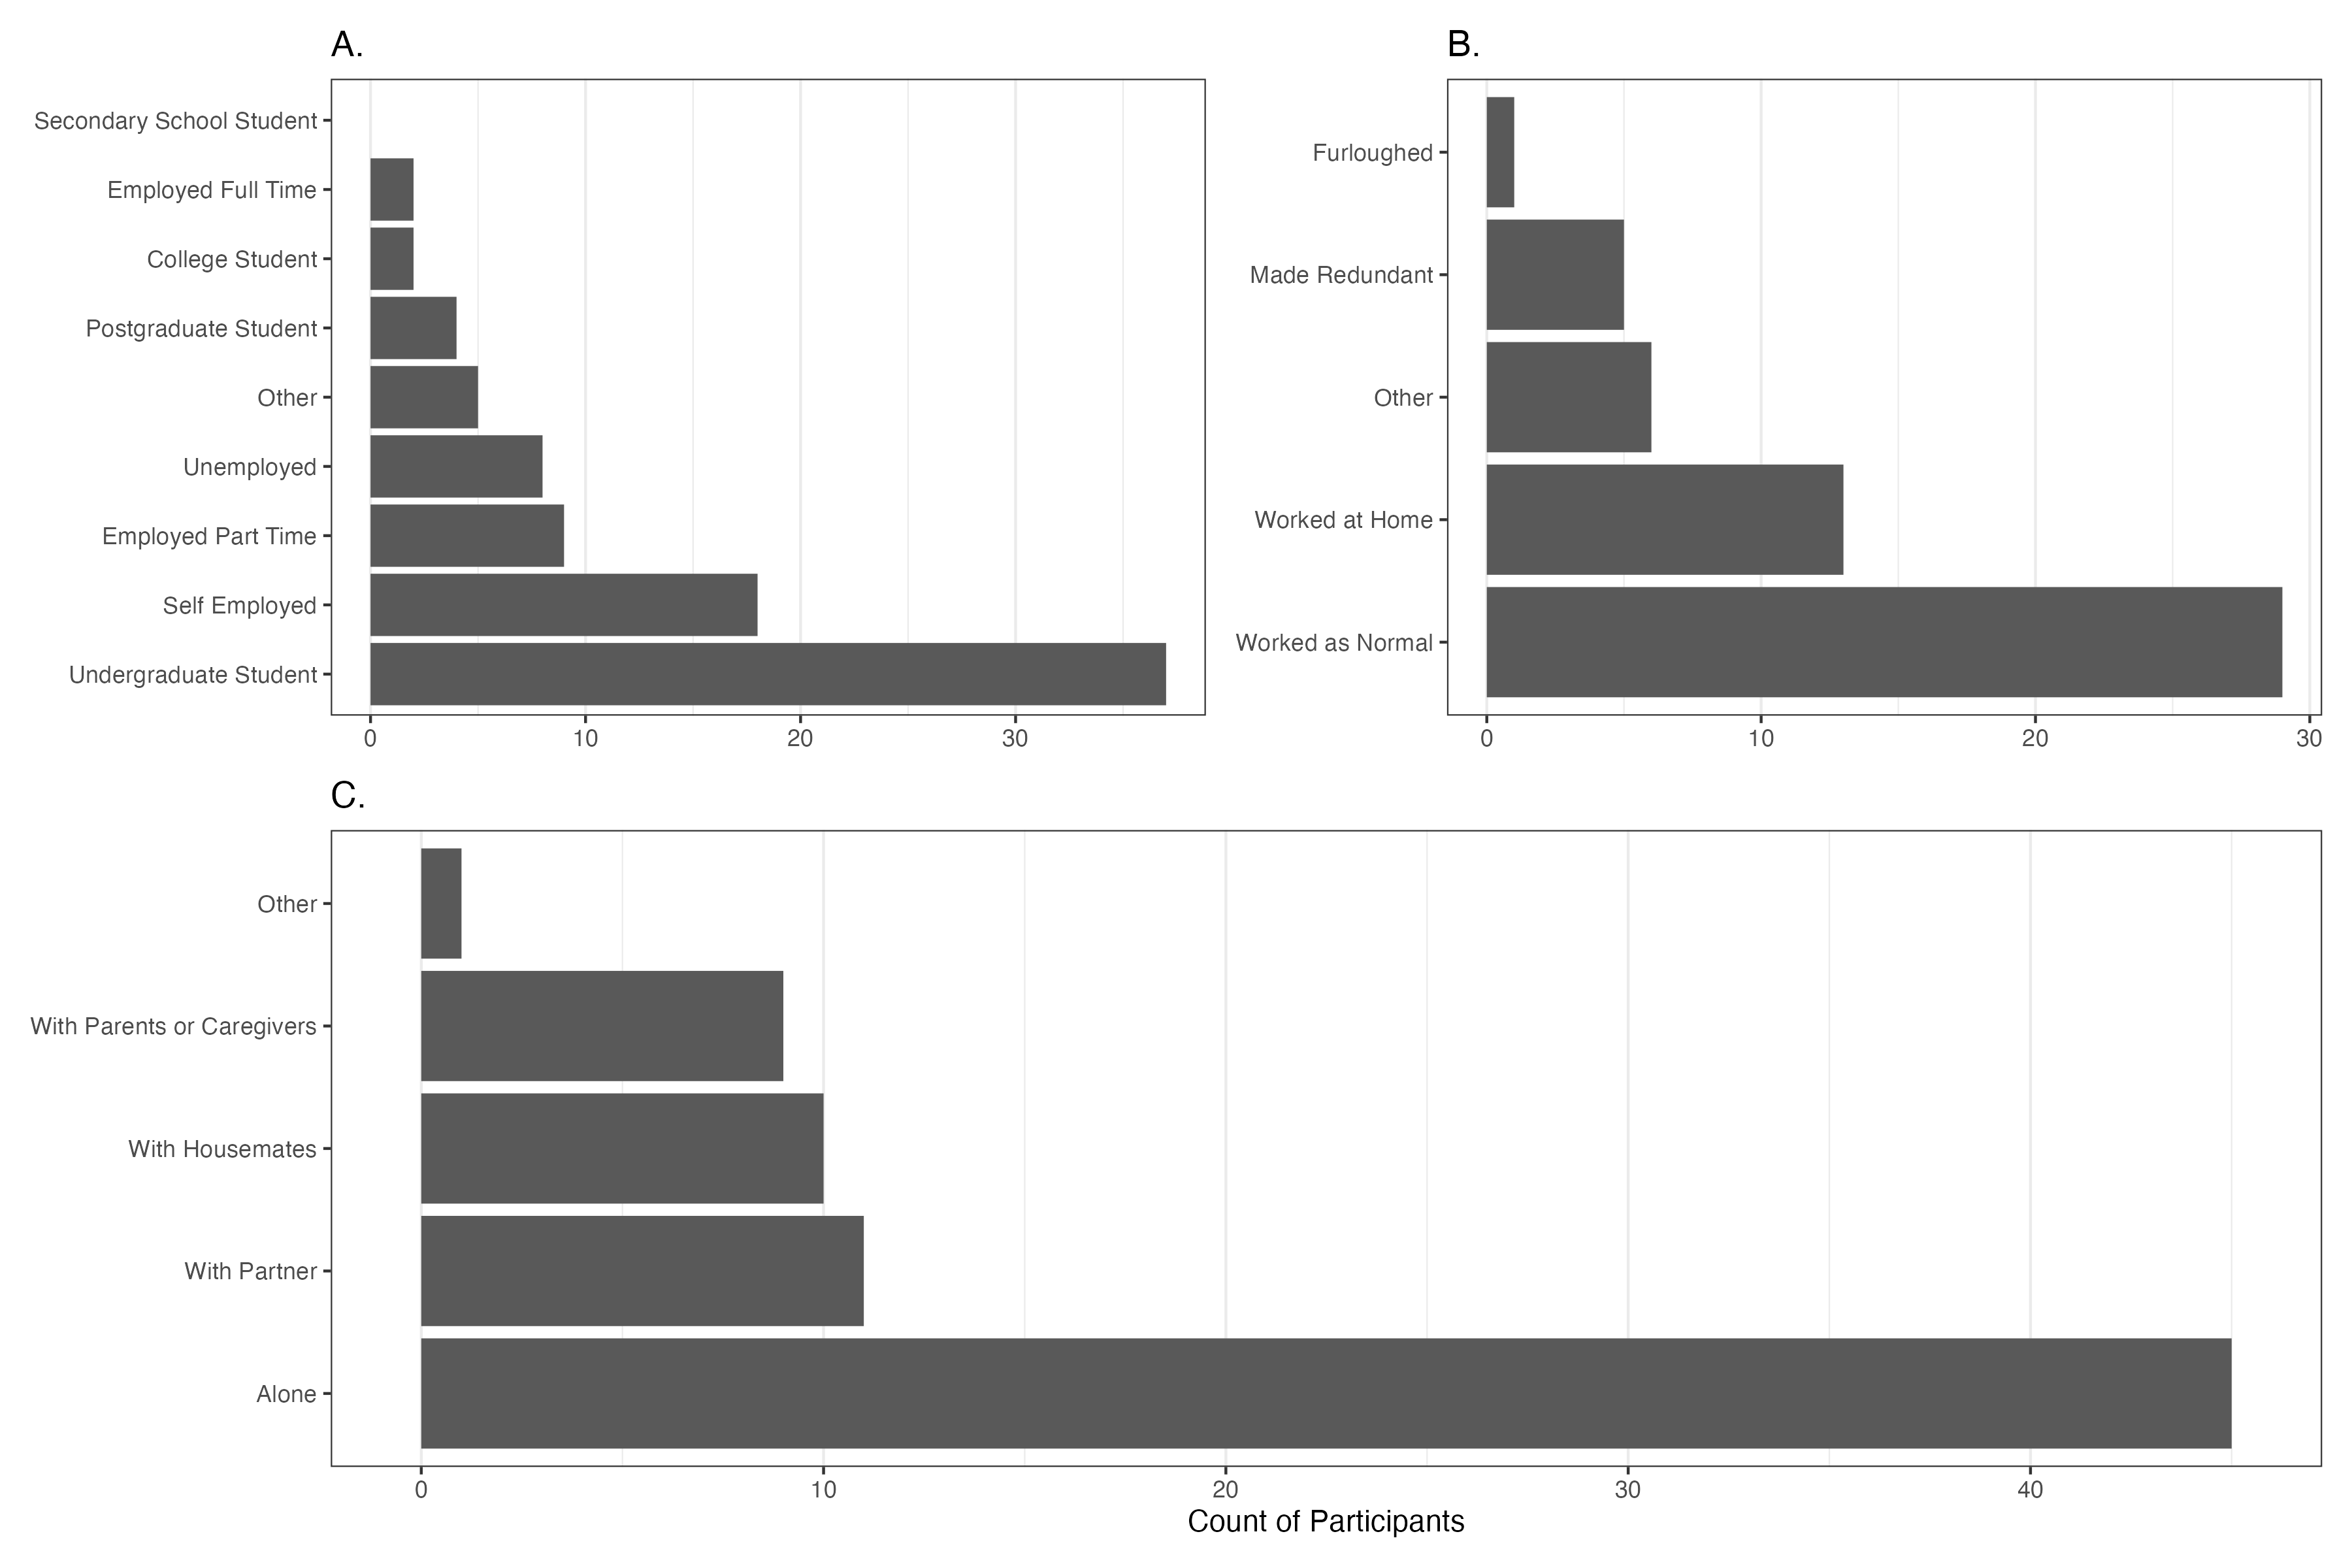
\includegraphics[width=0.9\linewidth]{/Users/glennwilliams/Dropbox/GitHub/covid-gaming/03_plots/situation_combined} 

}

\caption{Count of participants by self-reported (a) employment status, (b) lockdown work situation, and (c) living situation.}\label{fig:situations-plot}
\end{figure*}

\hypertarget{materials}{%
\subsection{Materials}\label{materials}}

A little info here.

\hypertarget{procedure}{%
\subsection{Procedure}\label{procedure}}

\hypertarget{data-analysis}{%
\subsection{Data analysis}\label{data-analysis}}

We used R (Version 4.0.3; R Core Team, 2020) and the R-packages \emph{BayesFactor} (Version 0.9.12.4.2; Morey \& Rouder, 2018), \emph{brms} (Version 2.14.4; Bürkner, 2017, 2018), \emph{coda} (Version 0.19.4; Plummer, Best, Cowles, \& Vines, 2006), \emph{dplyr} (Version 1.0.2; Wickham et al., 2020), \emph{english} (Version 1.2.5; Fox, Venables, Damico, \& Salverda, 2020), \emph{factoextra} (Version 1.0.7; Kassambara \& Mundt, 2020), \emph{flextable} (Version 0.6.3; Gohel, 2021), \emph{forcats} (Version 0.5.0; Wickham, 2020a), \emph{ggforce} (Version 0.3.3; Pedersen, 2021), \emph{ggplot2} (Version 3.3.2; Wickham, 2016), \emph{here} (Version 0.1; Müller, 2017), \emph{interactions} (Version 1.1.3; Long, 2019), \emph{janitor} (Version 2.0.1; Firke, 2020), \emph{kableExtra} (Version 1.3.4.9000; Zhu, 2020), \emph{lubridate} (Version 1.7.9; Grolemund \& Wickham, 2011), \emph{Matrix} (Version 1.2.18; Bates \& Maechler, 2019), \emph{mclust} (Version 5.4.7; Scrucca, Fop, Murphy, \& Raftery, 2016), \emph{modelr} (Version 0.1.8; Wickham, 2020b), \emph{papaja} (Version 0.1.0.9997; Aust \& Barth, 2020), \emph{patchwork} (Version 1.0.1; Pedersen, 2020), \emph{psych} (Version 2.0.8; Revelle, 2020), \emph{purrr} (Version 0.3.4; Henry \& Wickham, 2020), \emph{raincloudplots} (Version 0.2.0; person), 2021), \emph{Rcpp} (Version 1.0.5; Eddelbuettel \& François, 2011; Eddelbuettel \& Balamuta, 2017), \emph{readr} (Version 1.3.1; Wickham, Hester, \& Francois, 2018), \emph{stringr} (Version 1.4.0; Wickham, 2019), \emph{tibble} (Version 3.1.0; Müller \& Wickham, 2020), \emph{tidybayes} (Version 2.3.1; Kay, 2020), \emph{tidyr} (Version 1.1.2; Wickham, 2020c), and \emph{tidyverse} (Version 1.3.0; Wickham, Averick, et al., 2019) for all our analyses.

\hypertarget{results}{%
\section{Results}\label{results}}

Intro to the results and this plot.

\begin{figure*}[!htbp]

{\centering 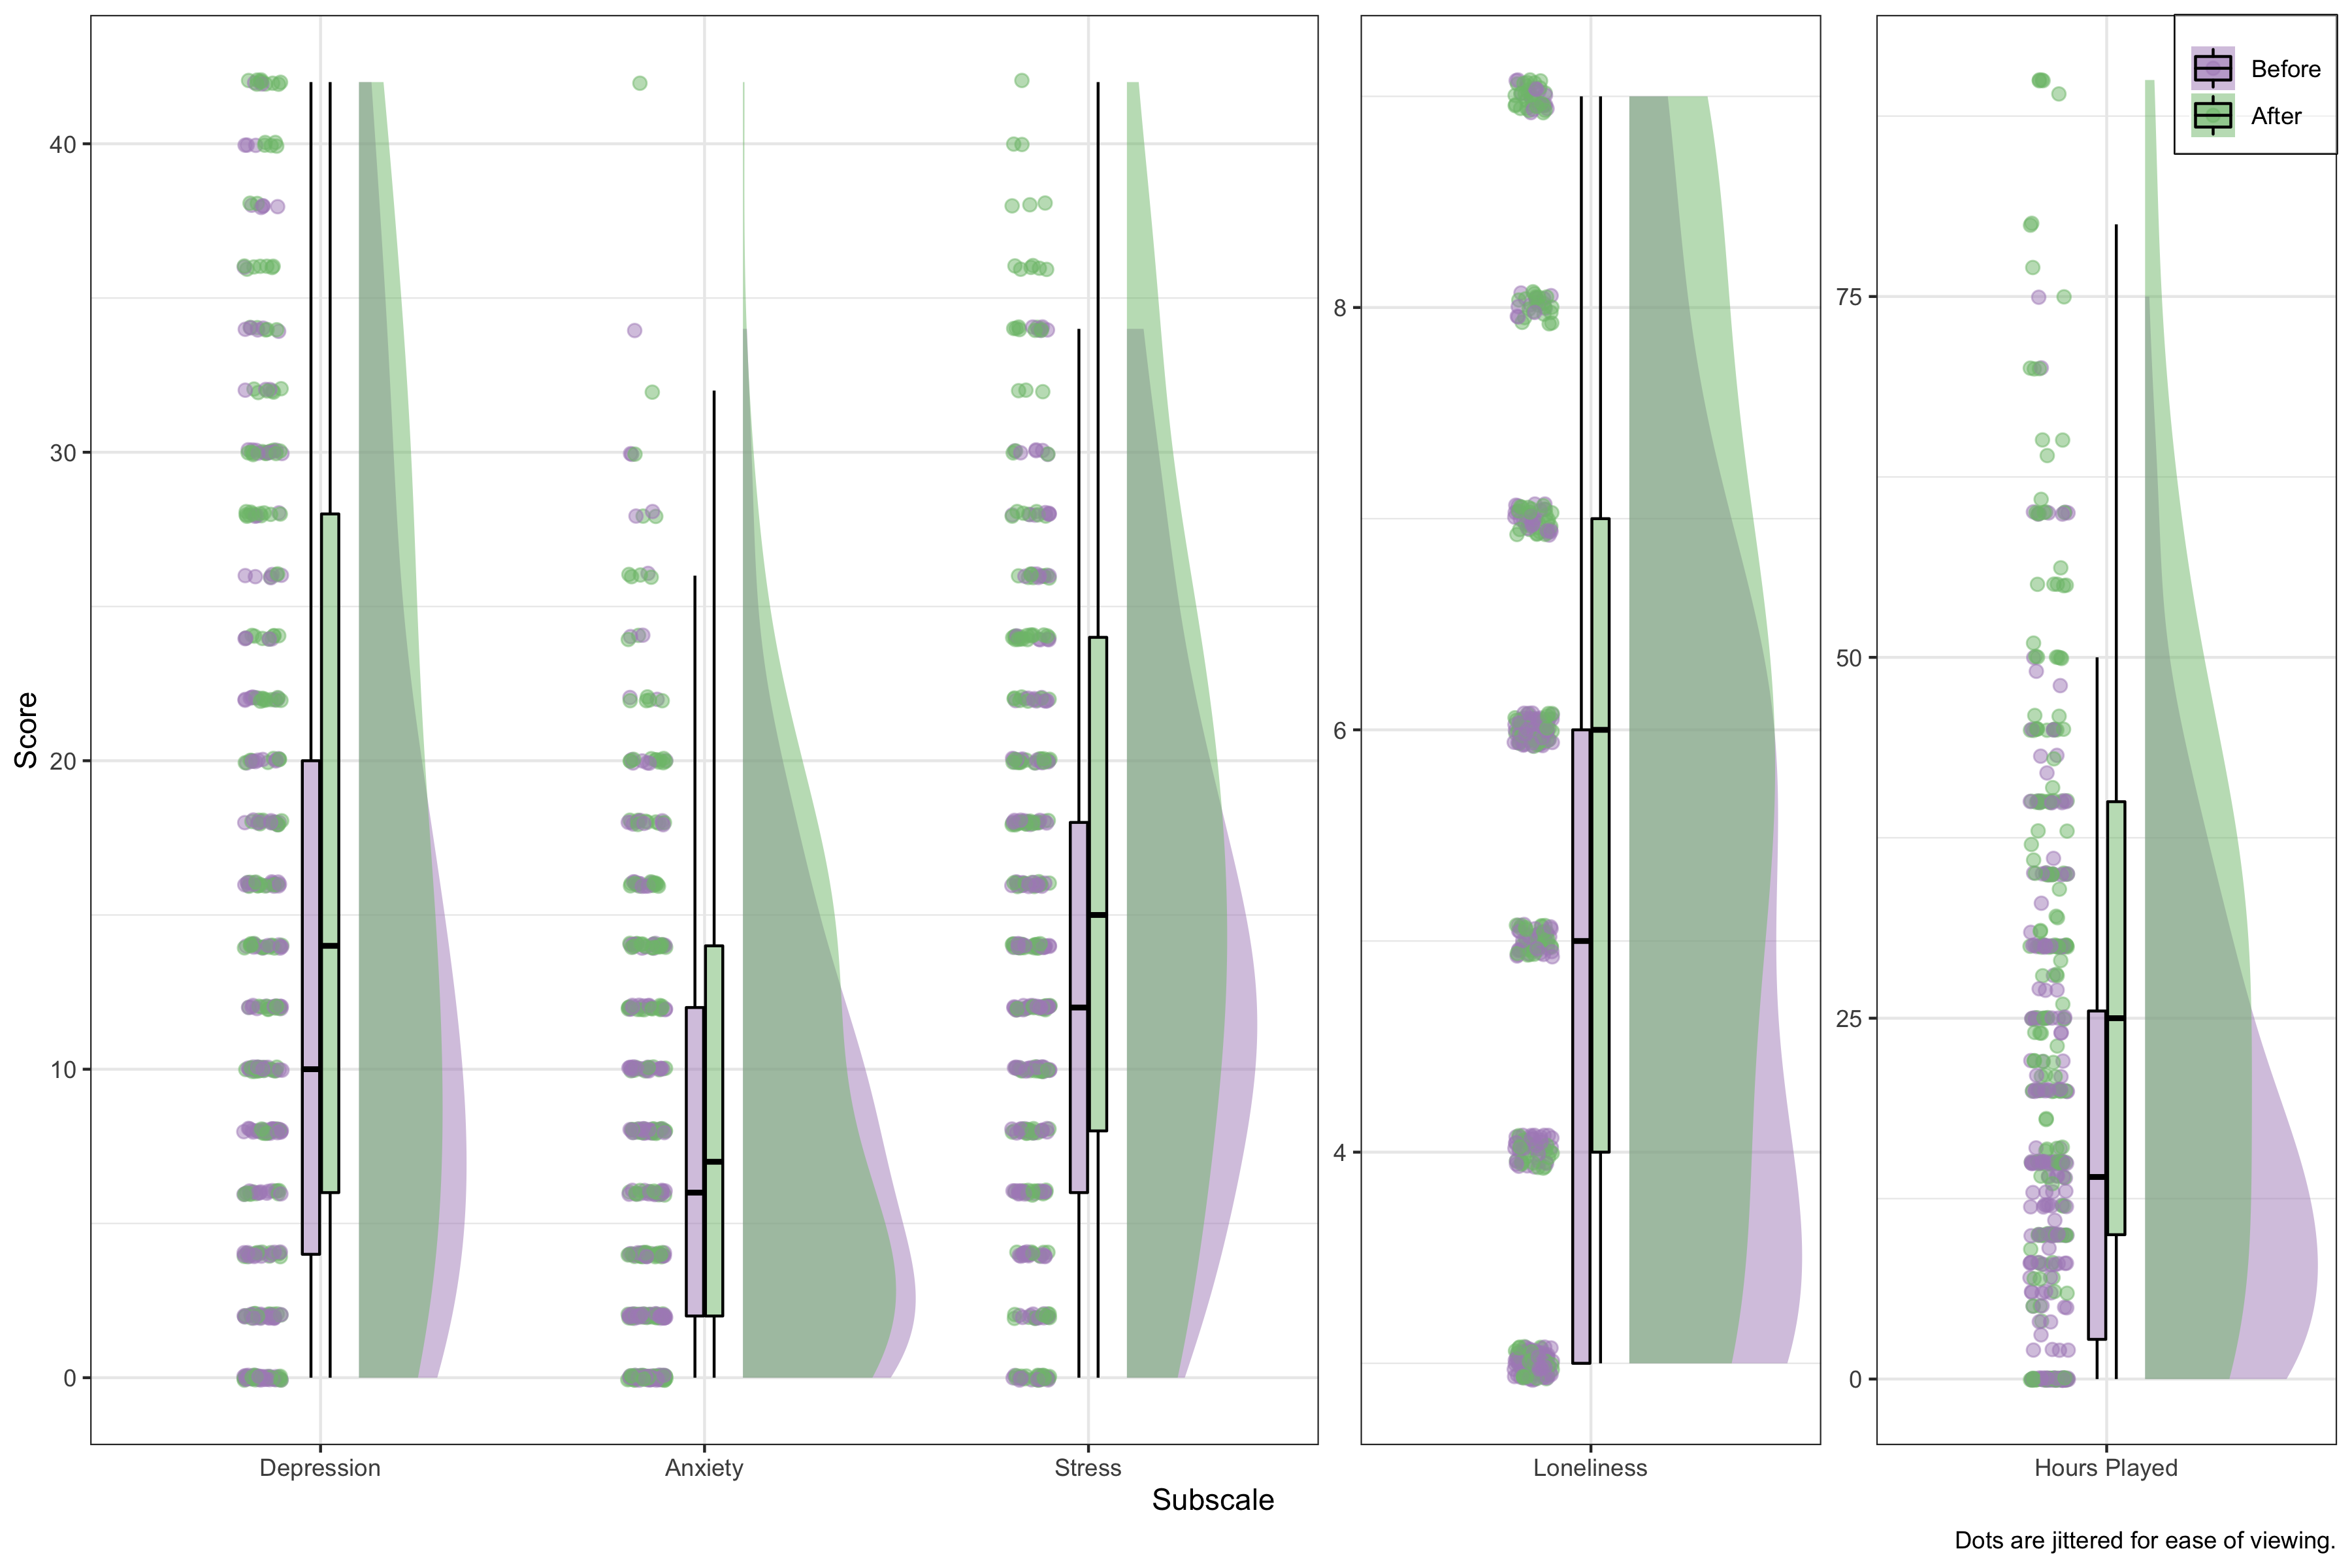
\includegraphics[width=0.9\linewidth]{/Users/glennwilliams/Dropbox/GitHub/covid-gaming/03_plots/mh_raincloud} 

}

\caption{Mental health outcomes for the depression, anxiety, stress, and loneliness along with total hours played before and during lockdown. Dots represent individual participants' (jittered) scores.}\label{fig:mh-raincloud-plot}
\end{figure*}

We used the \texttt{BayesFactor} R-package to calculate the Bayes factor for the evidence in support of an increase in hours played after lockdown. The model used a default \(Cauchy(0, 0.707)\) prior and estimated the posterior median and 95\% credible intervals using 1000 posterior samples. We found evidence in support of the alternative model (i.e.~of a difference in means) when compared to the null model (i.e.~no difference in means), \(BF_{10}\) \textgreater{} 1,000,000 (± 0\%), with posterior summaries showing an average increase in total hours played of 12.31 (\emph{SD} = 1.16, 95\% CI = {[}10.01, 14.50{]}). Having established that there was a general increase in hours spent gaming after lockdown we next established the role of total hours spent gaming on mental health outcomes.

\hypertarget{the-impact-of-hours-played-before-and-after-lockdown-on-mental-health-outcomes}{%
\subsection{The Impact of Hours Played Before and After Lockdown on Mental Health Outcomes}\label{the-impact-of-hours-played-before-and-after-lockdown-on-mental-health-outcomes}}

We took the data from the DASS questionnaire and loneliness questionnaire ratings before and after lockdown and combined these with hours played before and after lockdown. Given the data are generated from three Likert-style questionnaire responses per subscale, added together and multiplied by two, responses are thus strictly positive integers. This required fitting the data to cumulative models using a logit link function.

We fitted these models separately for each sub-scale of the DASS and for loneliness using the \texttt{brm} function in brms, estimating the effect of hours played in video games, time (pre- and post-lockdown), and the interaction between them. The categorical fixed effect of time was sum-coded (before = -1, after = 1) while the continuous fixed effect of total hours played was z-transformed. As a result, the intercept represents the grand mean and regression coefficients represent the impact of lockdown on mental health outcomes across the average hours played (i.e.~a main effect of time), the impact of hours played across the average of both time points (i.e.~a main effect of hours played), and their interaction. All models contained random intercepts per participant. Models used a \(Normal(0, 50)\) prior on the intercept, a \(Normal(0, 5)\) prior on the slope terms, and an \(Exponential(1)\) prior on the standard deviation term. We evaluate the evidence in support of the null hypothesis for each paramter estimate (i.e.~for a point-null effect of 0) using Bayes factors calculated using the Savage Savage-Dickey density ratio using the \texttt{hypothesis} function in brms. The population-level (fixed effect) parameter are reported in the Appendix on the log scale and backtransformed to the natural (i.e.~rating) scale.

The population-level estimates for mental health outcomes based on total hours played before and after lockdown are shown for each model in Figure ~\ref{fig:mh-main-predictions-plot}.

\begin{figure*}[!htbp]

{\centering 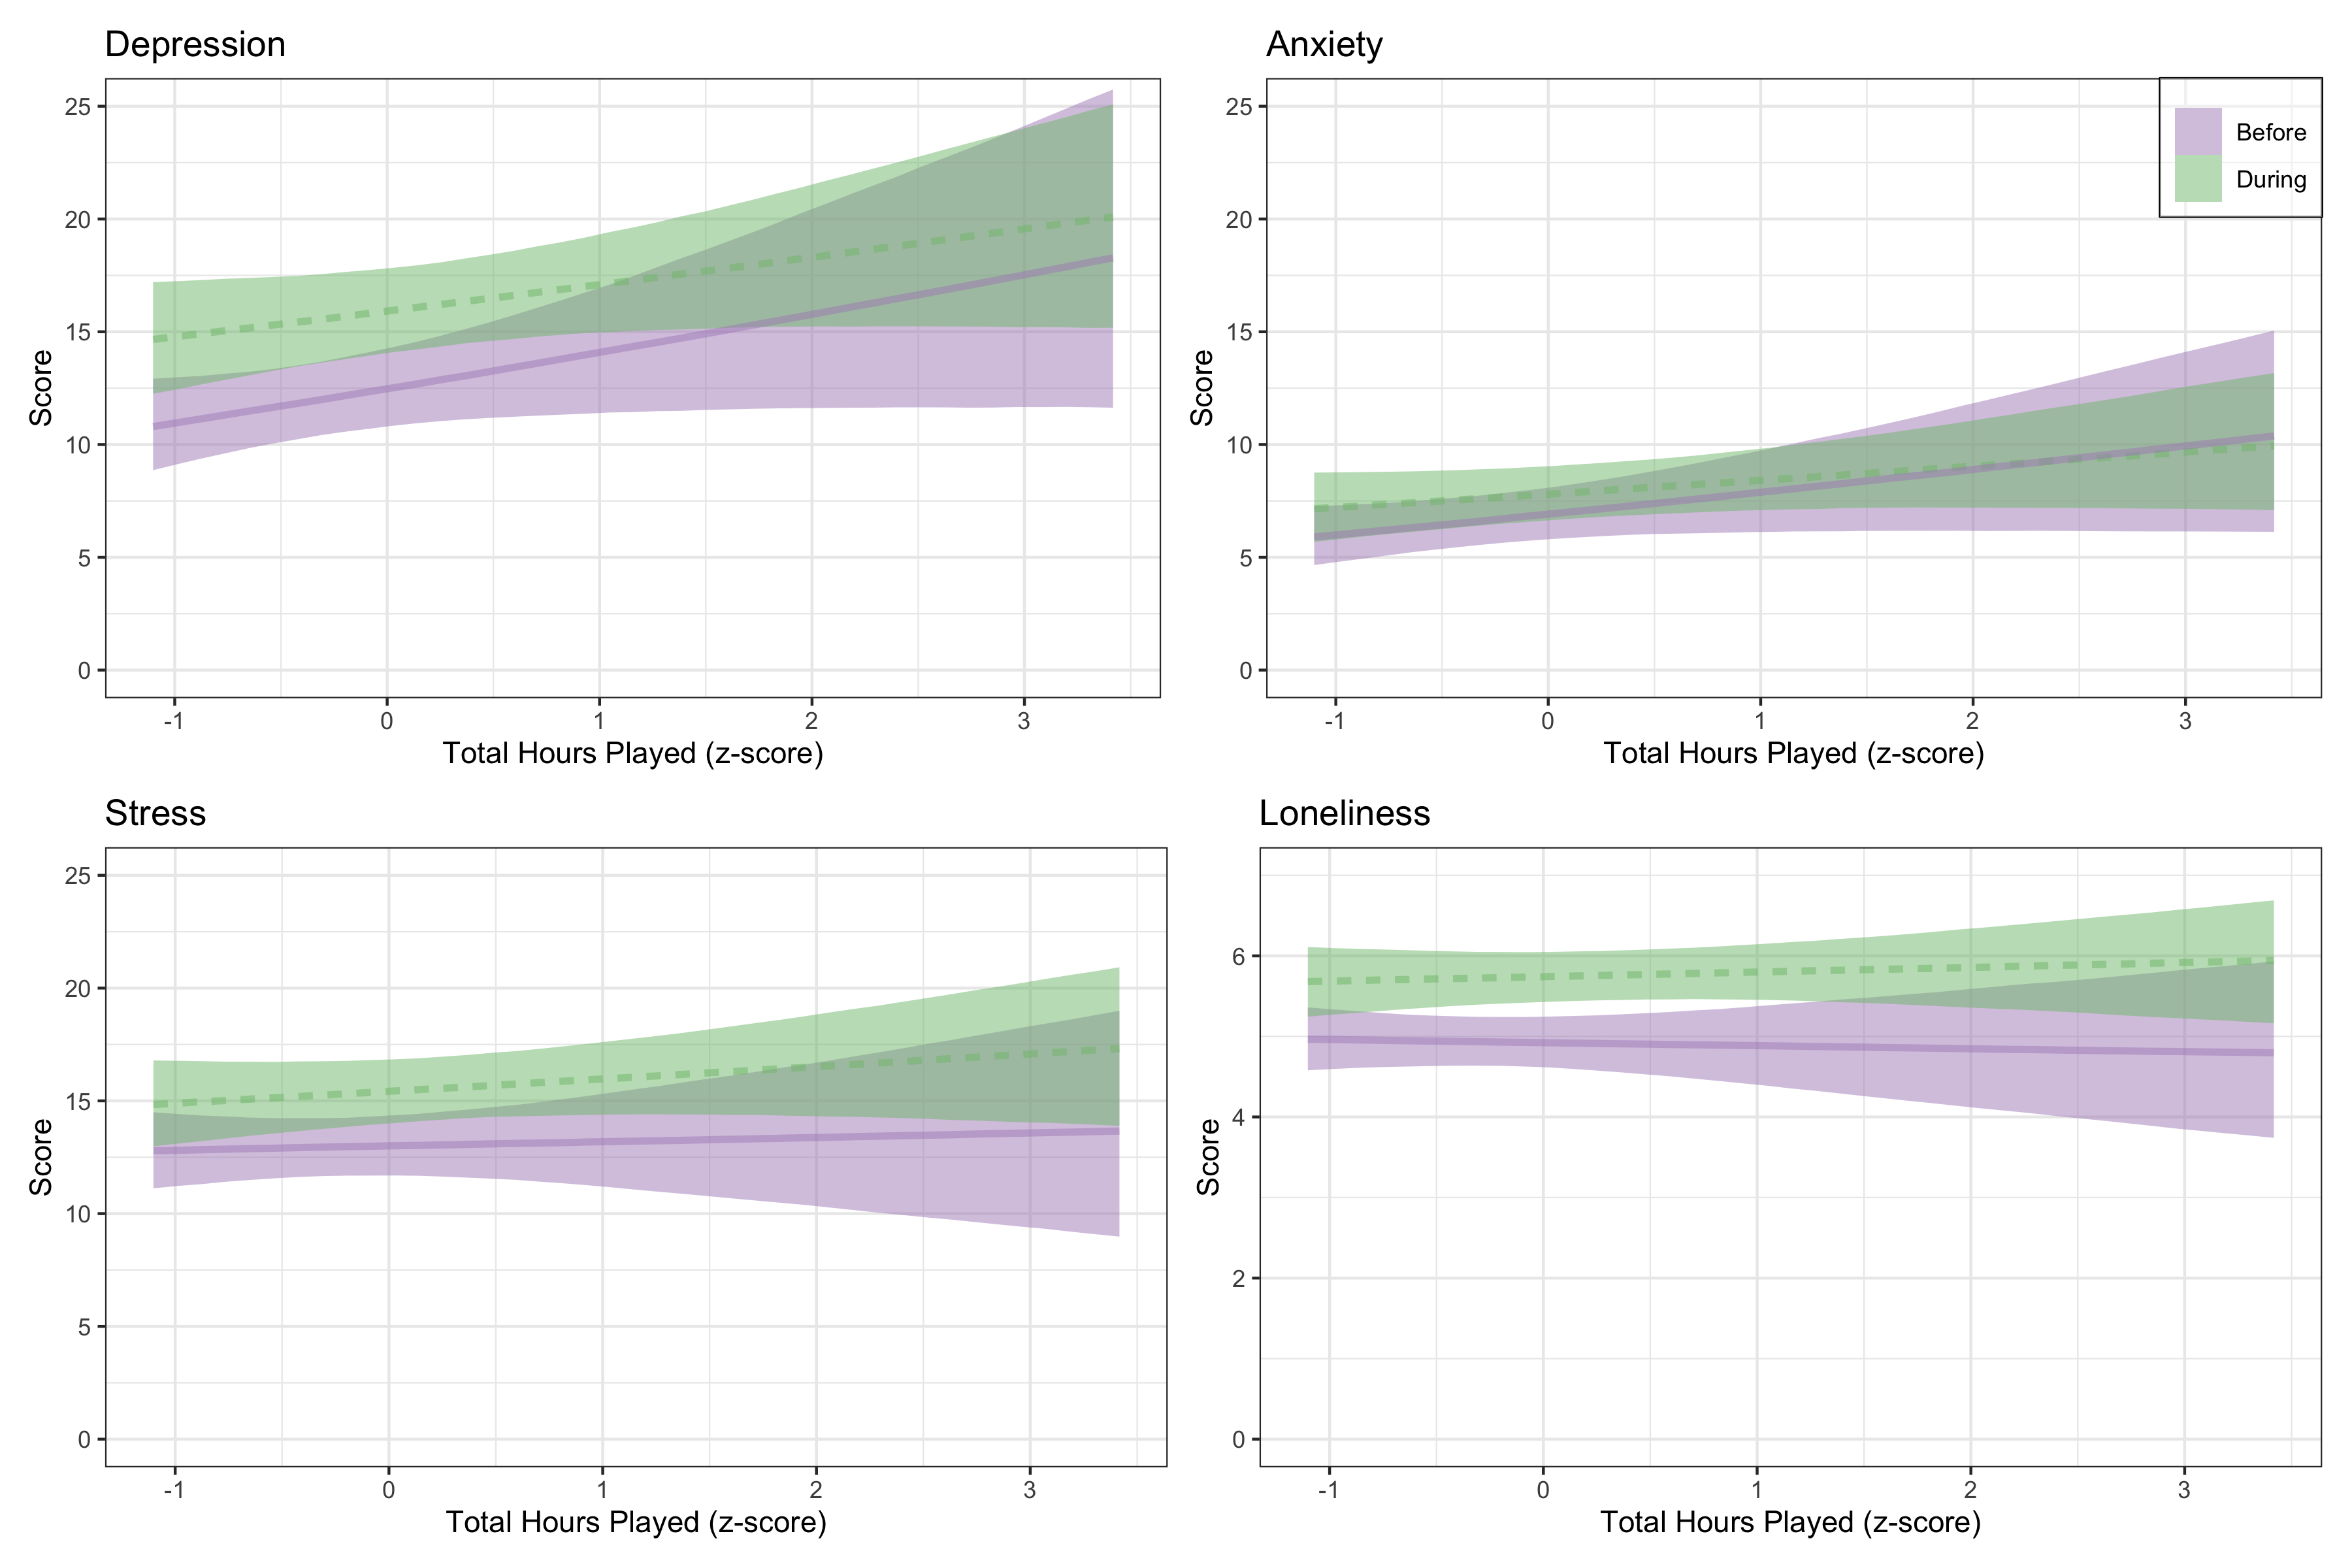
\includegraphics[width=0.9\linewidth]{/Users/glennwilliams/Dropbox/GitHub/covid-gaming/03_plots/mh_main_predictions} 

}

\caption{Mental health outcomes for the depression, anxiety, stress, and loneliness measures as a function of total hours played before and during lockdown. Lines and ribbons indicate the posterior median ± 95\% credible intervals.}\label{fig:mh-main-predictions-plot}
\end{figure*}

Table~\ref{tab:dass-bayes-pre-post} shows the population-level parameter estimates, their standard error, and 95\% credible intervals on the log scale for both main effects and their interaction for each model.

\begin{table*}[tbp]

\begin{center}
\begin{threeparttable}

\caption{\label{tab:dass-bayes-pre-post}Bayes factors for the depression, anxiety, stress, and loneliness models evaluating evidence in support of the point null hypothesis that each parameter estimate is equal to zero.}

\begin{tabular}{lllll}
\toprule
Parameter & \multicolumn{1}{c}{$Est.$} & \multicolumn{1}{c}{$SE$} & \multicolumn{1}{c}{95\% CI} & \multicolumn{1}{c}{$BF_{01}$}\\
\midrule
Depression &  &  &  & \\
\ \ \ Time & 0.48 & 0.14 & [0.22, 0.75] & 0.10\\
\ \ \ Total Hours & 0.33 & 0.22 & [-0.10, 0.75] & 7.20\\
\ \ \ Time by Hours & -0.06 & 0.14 & [-0.34, 0.20] & 34.01\\
Anxiety &  &  &  & \\
\ \ \ Time & 0.18 & 0.14 & [-0.09, 0.44] & 17.10\\
\ \ \ Total Hours & 0.37 & 0.22 & [-0.07, 0.80] & 5.48\\
\ \ \ Time by Hours & -0.08 & 0.13 & [-0.35, 0.18] & 32.12\\
Stress &  &  &  & \\
\ \ \ Time & 0.50 & 0.13 & [0.24, 0.76] & 0.00\\
\ \ \ Total Hours & -0.07 & 0.21 & [-0.50, 0.37] & 21.89\\
\ \ \ Time by Hours & 0.11 & 0.13 & [-0.14, 0.37] & 26.80\\
Loneliness &  &  &  & \\
\ \ \ Time & 0.70 & 0.15 & [0.42, 1.02] & 0.00\\
\ \ \ Total Hours & -0.07 & 0.22 & [-0.52, 0.36] & 22.96\\
\ \ \ Time by Hours & 0.04 & 0.15 & [-0.24, 0.33] & 33.41\\
\bottomrule
\addlinespace
\end{tabular}

\begin{tablenotes}[para]
\normalsize{\textit{Note.} Higher values indicate support for the null hypothesis while lower numbers indicate support for the alternative hypothesis (i.e. of a non-null effect).}
\end{tablenotes}

\end{threeparttable}
\end{center}

\end{table*}

We found evidence against the null for the effect of time in the Depression, Stress, and Loneliness models where parameter estimates and credible intervals show an increase in negative outcomes on these scales when going from the pre-lockdown to lockdown periods. The Anxiety model showed evidence in support of the null whereby there was no reliable change in anxiety between the pre-lockdown and lockdown periods. In all models, we found evidence in support of the null hypothesis for the impact of total hours playing games and the interaction between time (pre-lockdown and during lockdown) and the total hours playing games on mental health outcomes.

We next explored the effect of the change in total hours playing games before and during lockdown on the mental health outcomes during lockdown. Here, hours played after were subtracted from hours played before. Models were again fitted separately for each subscale in brms using the \texttt{brm} function. Here, the data were fitted using a Gaussian model (identity link function), with the fixed effect of total hours played during lockdown. Models used a \(Normal(0, 5)\) prior on the intercept, a \(Normal(0, 1)\) prior on the slope term, and an \(Exponential(1)\) prior on the sigma term. Effects were evaluated using the same methods outlined above.

The population-level predictions for the change in mental health outcomes as a measure of total hours played during lockdown are shown for each model in Figure ~\ref{fig:mh-diff-l-plot}.

\begin{figure*}[!htbp]

{\centering 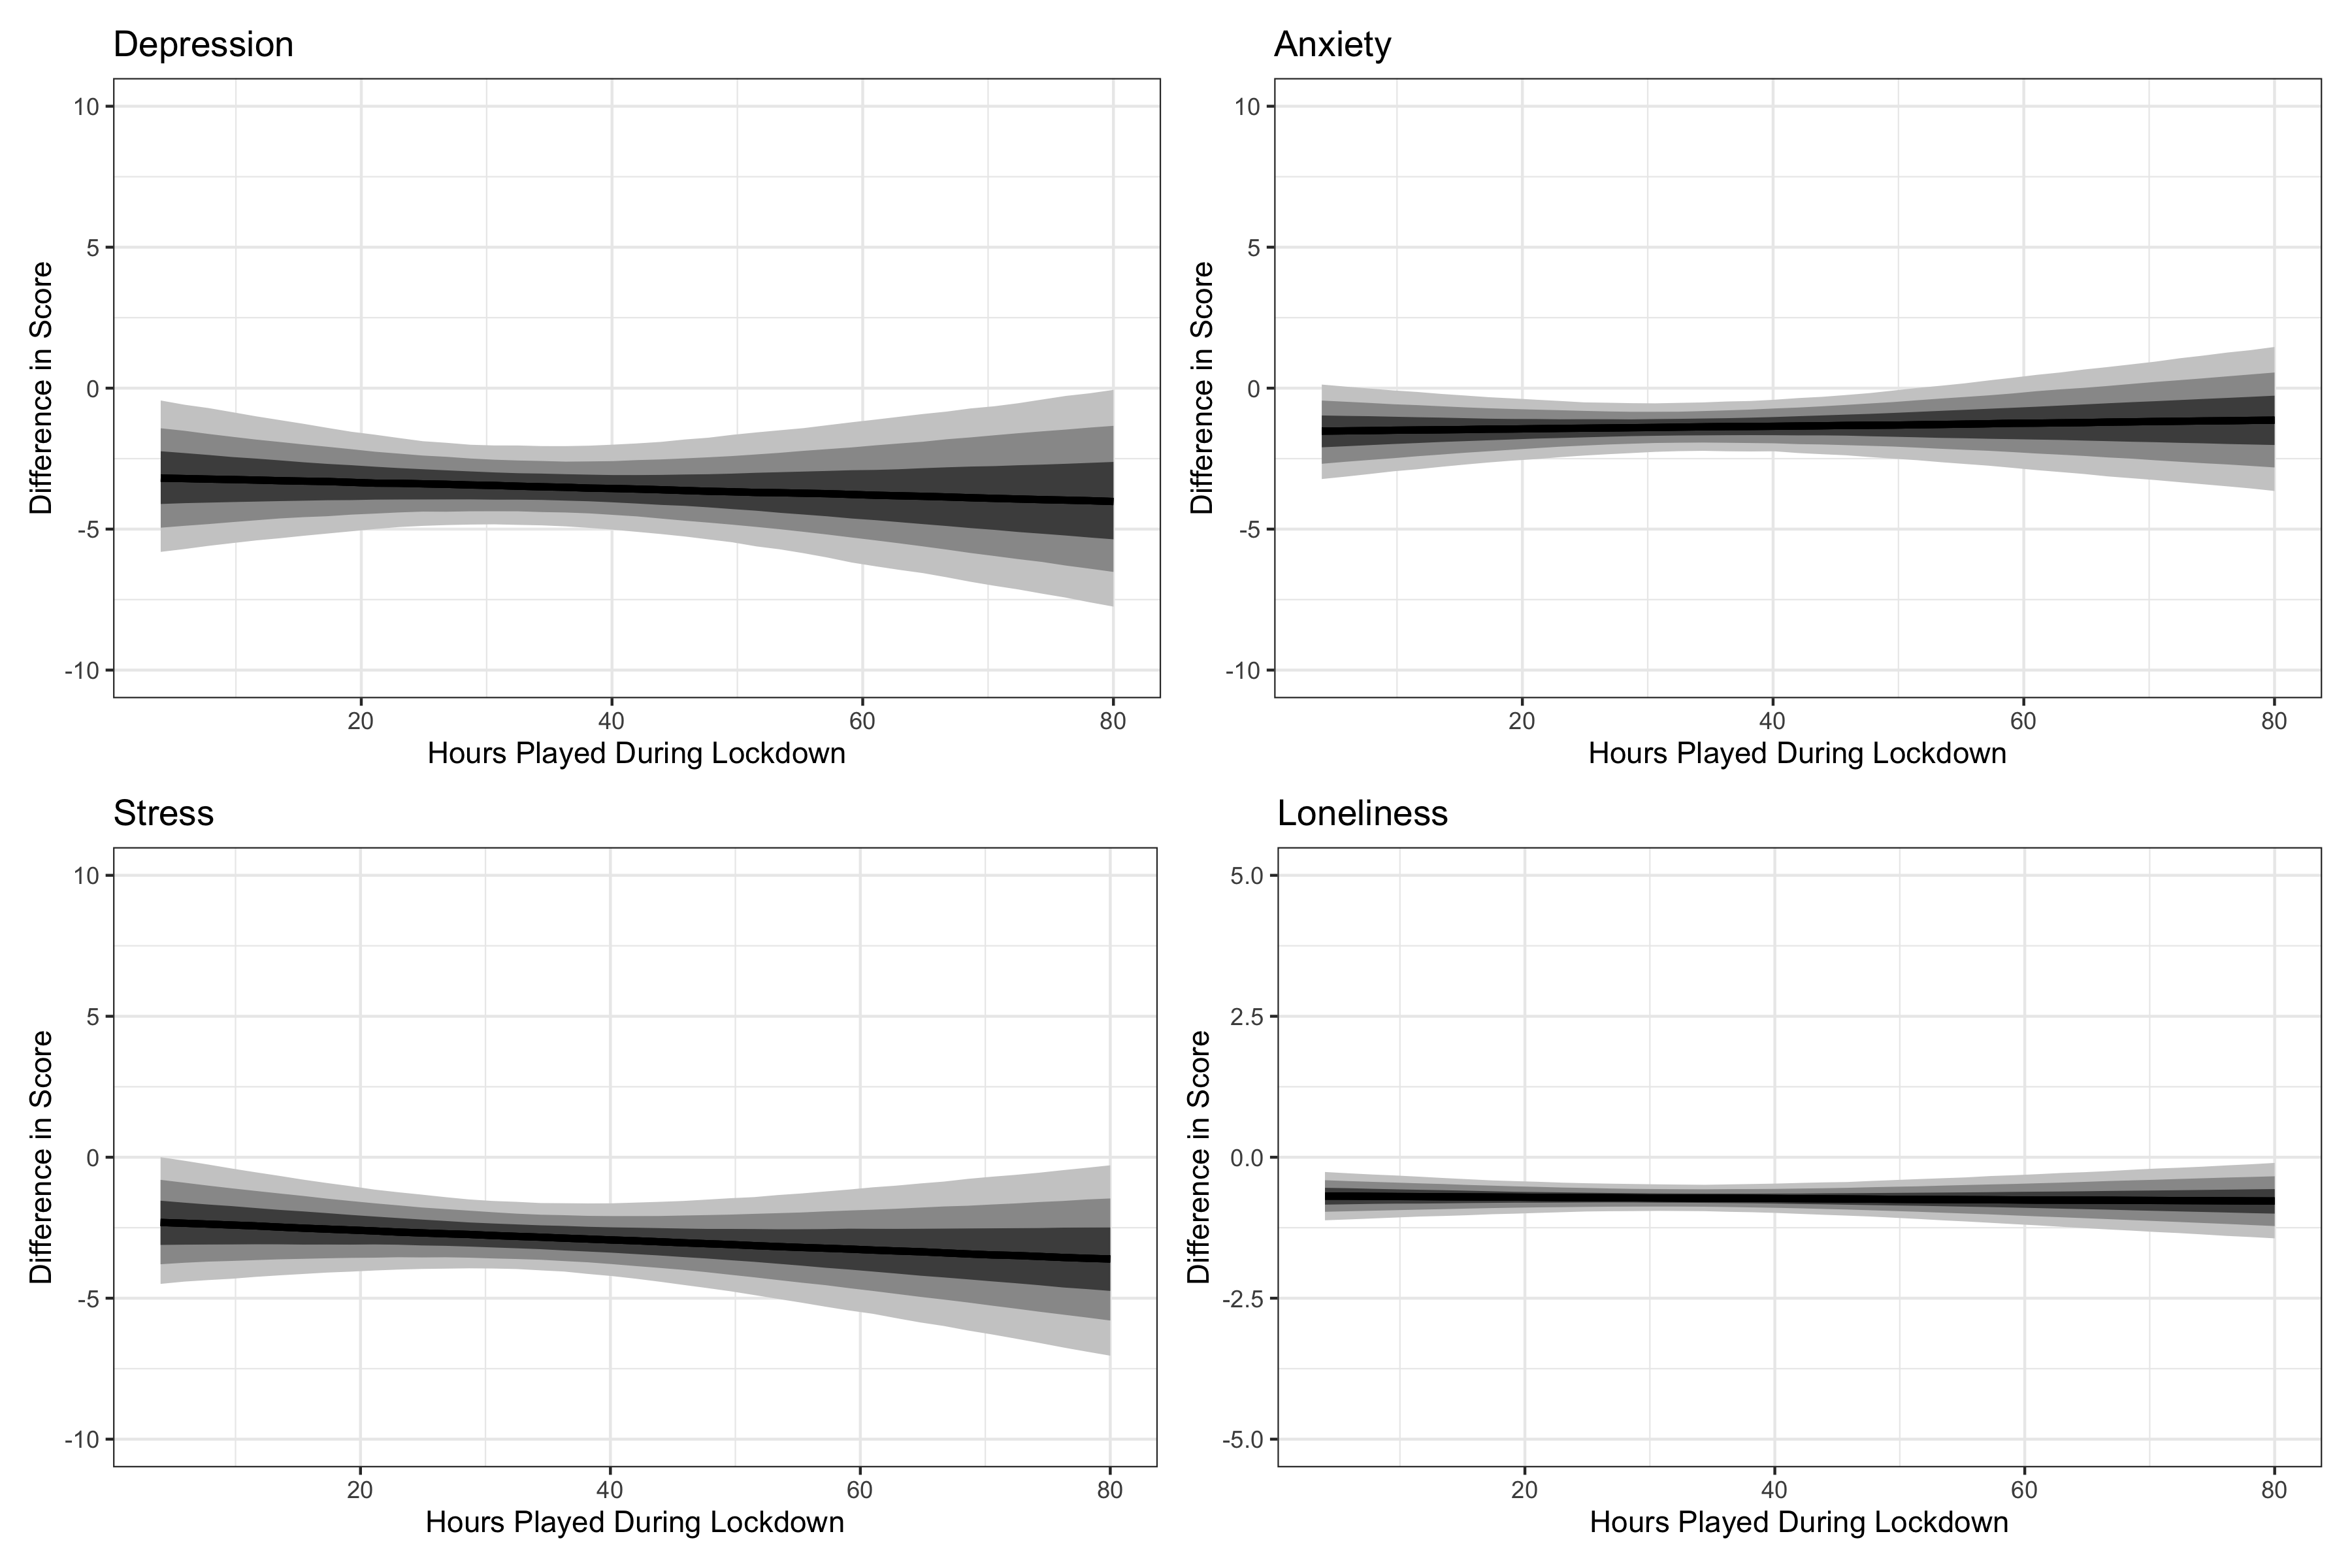
\includegraphics[width=0.9\linewidth]{/Users/glennwilliams/Dropbox/GitHub/covid-gaming/03_plots/mh_diff_l} 

}

\caption{Change in mental health outcomes for the depression, anxiety, stress, and loneliness measures as a function of the total hours played during lockdown. Lines indicate the posterior median ± 50\%, 80\%, and 95\% credible intervals.}\label{fig:mh-diff-l-plot}
\end{figure*}

Table~\ref{tab:dass-bayes-l-diff} shows the population-level parameter estimates, their standard error, and 95\% credible intervals on the log scale for both main effects and their interaction for each model.

\begin{table*}[tbp]

\begin{center}
\begin{threeparttable}

\caption{\label{tab:dass-bayes-l-diff}Bayes factors for the depression, anxiety, stress, and loneliness models evaluating evidence in support of the point null hypothesis that the difference in hours played has no impact on mental health outcomes during lockdown.}

\begin{tabular}{lllll}
\toprule
Model & \multicolumn{1}{c}{$Est.$} & \multicolumn{1}{c}{$SE$} & \multicolumn{1}{c}{95\% CI} & \multicolumn{1}{c}{$BF_{01}$}\\
\midrule
Depression & -0.01 & 0.04 & [-0.09, 0.07] & 24.47\\
Anxiety & 0.01 & 0.03 & [-0.04, 0.06] & 36.84\\
Stress & -0.02 & 0.03 & [-0.08, 0.05] & 25.98\\
Loneliness & 0.00 & 0.01 & [-0.01, 0.01] & 161.74\\
\bottomrule
\addlinespace
\end{tabular}

\begin{tablenotes}[para]
\normalsize{\textit{Note.} Higher values indicate support for the null hypothesis while lower numbers indicate support for the alternative hypothesis (i.e. of a non-null effect).}
\end{tablenotes}

\end{threeparttable}
\end{center}

\end{table*}

Table~\ref{tab:dass-bayes-l-diff} shows evidence in support of the null hypothesis of no impact of change in hours played on mental health outcomes during lockdown for all subscales.

Finally, we explored the effect of the change in total hours playing games before and during lockdown on the difference in mental health outcomes pre-lockdown and during lockdown. Here, hours played after were subtracted from hours played before, and DASS outcomes after were (separately) subtracted from DASS outcomes before. Models were again fitted separately for each subscale in brms using the \texttt{brm} function using the same priors outlined in the models evaluating change in total hours playing games before and during lockdown on the mental health outcomes during lockdown. Here, the data were fitted using a Gaussian model (identity link function), with the fixed effect of difference in hours played. Effects were evaluated using the same methods outlined above.

The population-level estimates for the change in mental health outcomes as a measure of the difference in hours played before and after lockdown are shown for each model in Figure ~\ref{fig:mh-diff-plot}.

\begin{figure*}[!htbp]

{\centering 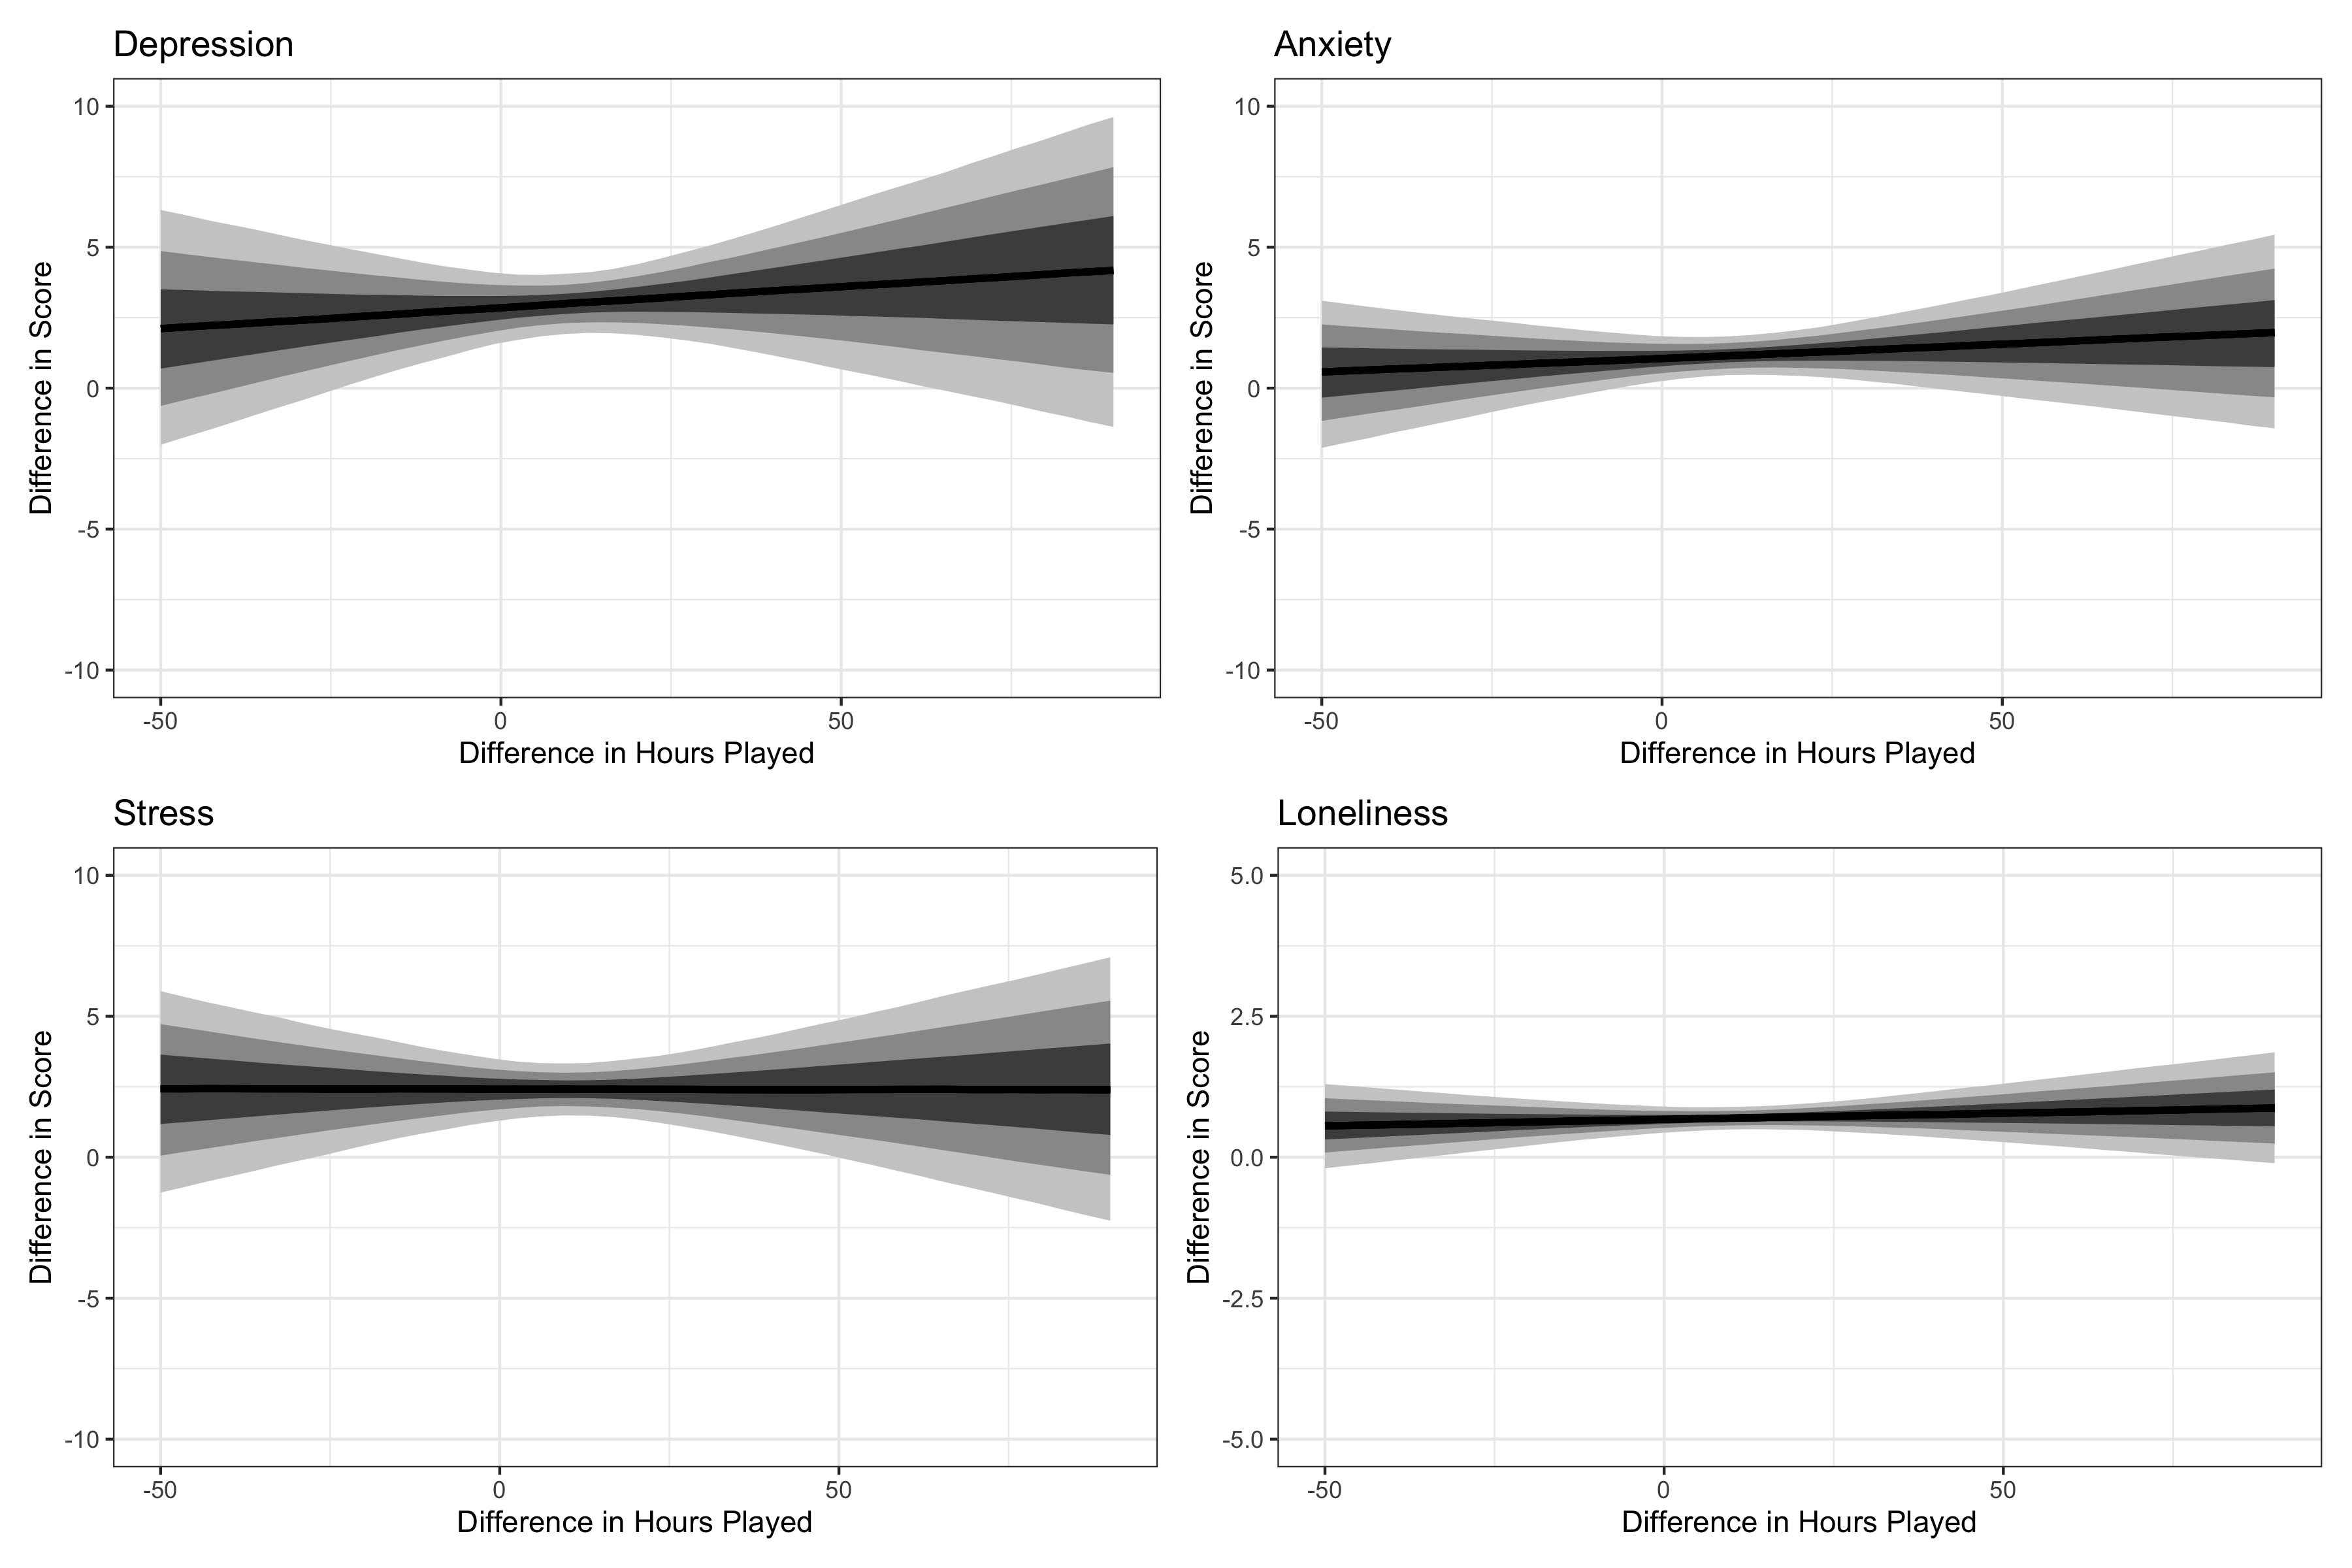
\includegraphics[width=0.9\linewidth]{/Users/glennwilliams/Dropbox/GitHub/covid-gaming/03_plots/mh_diff} 

}

\caption{Change in mental health outcomes for the depression, anxiety, stress, and loneliness measures as a function of the difference in hours played before and after lockdown. Lines indicate the posterior median ± 50\%, 80\%, and 95\% credible intervals.}\label{fig:mh-diff-plot}
\end{figure*}

Table~\ref{tab:dass-bayes-diff} shows the population-level parameter estimates, their standard error, and 95\% credible intervals on the log scale for both main effects and their interaction for each model.

\begin{table*}[tbp]

\begin{center}
\begin{threeparttable}

\caption{\label{tab:dass-bayes-diff}Bayes factors for the depression, anxiety, stress, and loneliness models evaluating evidence in support of the point null hypothesis that the difference in hours played has no impact on the change in mental health outcomes.}

\begin{tabular}{lllll}
\toprule
Model & \multicolumn{1}{c}{$Est.$} & \multicolumn{1}{c}{$SE$} & \multicolumn{1}{c}{95\% CI} & \multicolumn{1}{c}{$BF_{01}$}\\
\midrule
Depression & 0.02 & 0.05 & [-0.07, 0.12] & 16.98\\
Anxiety & 0.01 & 0.03 & [-0.06, 0.07] & 29.32\\
Stress & -0.02 & 0.04 & [-0.11, 0.06] & 20.62\\
Loneliness & 0.00 & 0.01 & [-0.02, 0.01] & 109.50\\
\bottomrule
\addlinespace
\end{tabular}

\begin{tablenotes}[para]
\normalsize{\textit{Note.} Higher values indicate support for the null hypothesis while lower numbers indicate support for the alternative hypothesis (i.e. of a non-null effect).}
\end{tablenotes}

\end{threeparttable}
\end{center}

\end{table*}

Table~\ref{tab:dass-bayes-diff} shows evidence in support of the null hypothesis of no impact in change in hours played on changes in mental health outcomes for all subscales.

WE COULD POTENTIALLY PUT CORRELATIONS HERE, BUT THEY DON'T SHOW ANYTHING THAT INTERESTING:

\begin{itemize}
\tightlist
\item
  metal health outcomes before lockdown are correlated.
\item
  hours played after is correlated with stress before.
\end{itemize}

\hypertarget{gaming-motivations}{%
\subsection{Gaming Motivations}\label{gaming-motivations}}

We explored the impact of gaming motivations on potential mental health outcomes. The pattern of gaming motivations is shown in Figure~\ref{fig:gaming-motivations-plot}. This shows that overall there are minor changes to motivations as a result of lockdown. Moreover, while amotivation and introjected regulation were overall quite low during both time periods, intrinsic motivation was high.

\begin{figure*}[!htbp]

{\centering 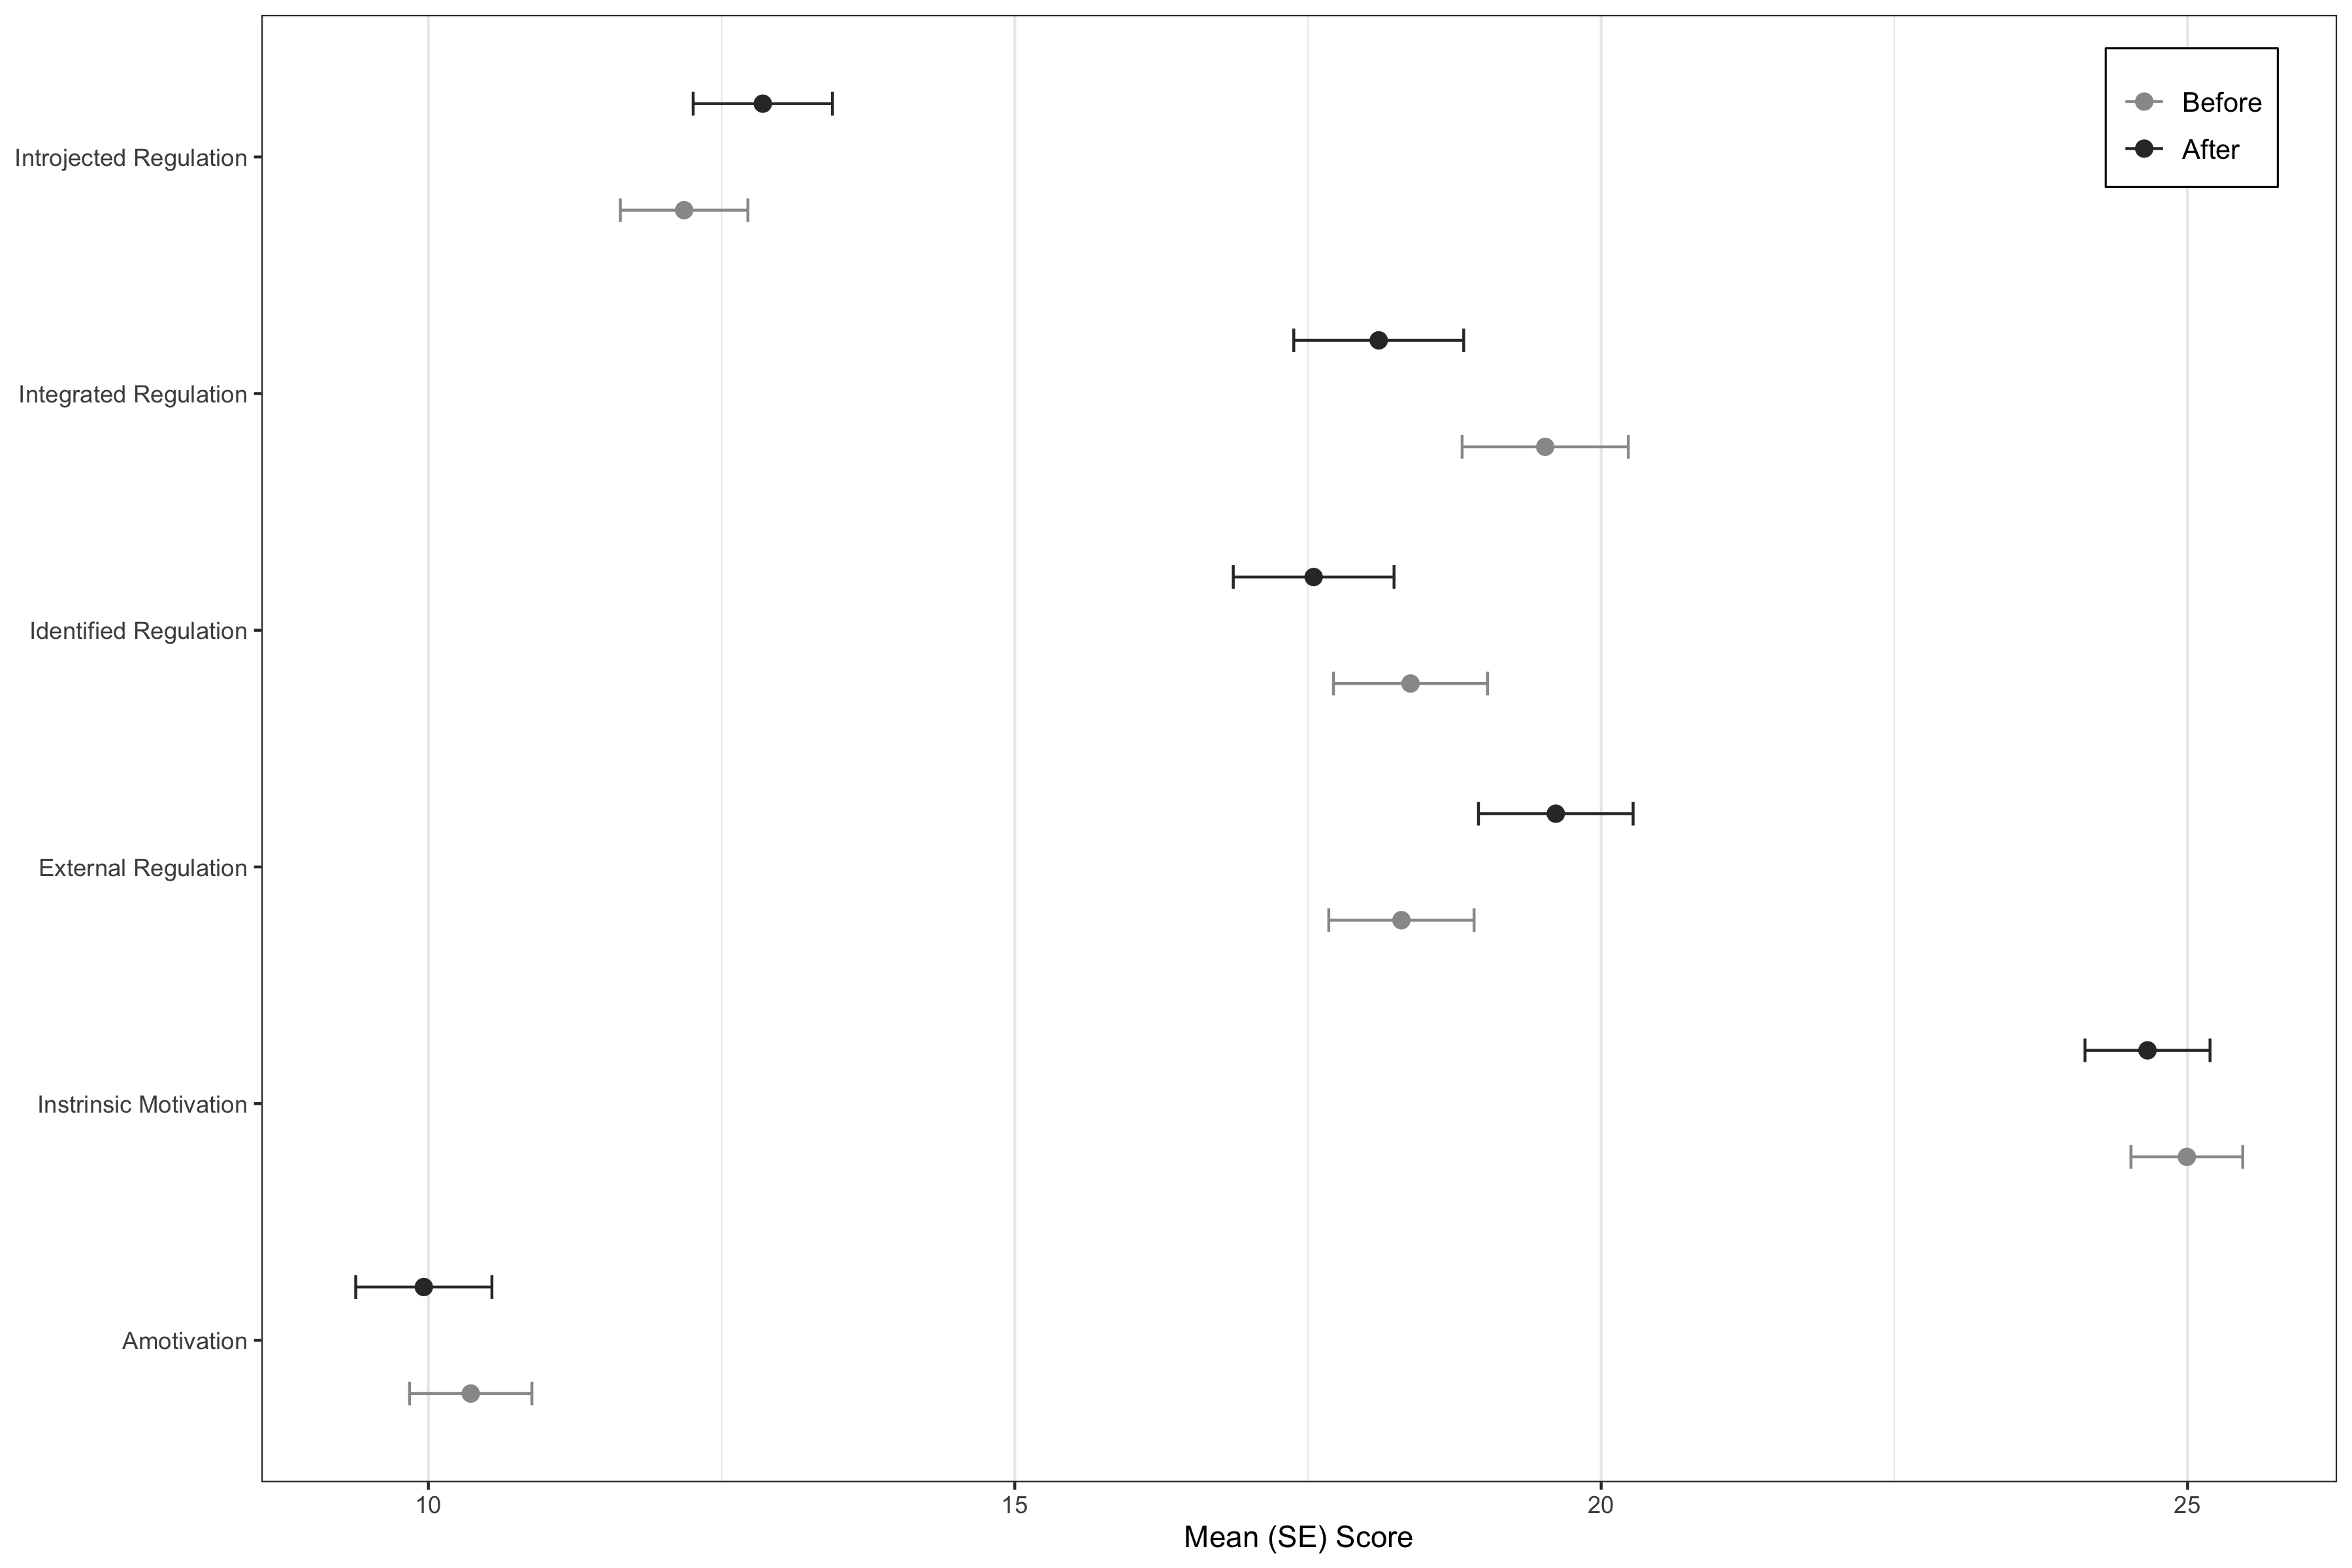
\includegraphics[width=0.9\linewidth]{/Users/glennwilliams/Dropbox/GitHub/covid-gaming/03_plots/gam_mean_se} 

}

\caption{ }\label{fig:gaming-motivations-plot}
\end{figure*}

We performed a series of Bayesian correlations using the \texttt{BayesFactor} R-package to calculate Bayes factors for the evidence in support of a correlation between mental health outcomes and gaming motivations. These correlations used a default, non-informative \(Beta(3, 3)\) prior. Posterior means and 95\% credible intervals using 1000 posterior samples. The result of these correlations is shown in Table~\ref{tab:motivation-correlations}.

\begin{table*}[tbp]

\begin{center}
\begin{threeparttable}

\caption{\label{tab:motivation-correlations}Correlation coefficients, 95\% credible intervals, and Bayes factors for the correlation between mental health outcomes during lockdown and gaming motivations before and after lockdown.}

\begin{tabular}{lllll}
\toprule
Outcome & \multicolumn{1}{c}{Amotivation Before} & \multicolumn{1}{c}{Amotivation After} & \multicolumn{1}{c}{Instrinsic Motivation Before} & \multicolumn{1}{c}{Instrinsic Motivation After}\\
\midrule
Depression After & \makecell[c]{0.29 [0.16, 0.43], \\$BF_{10}$ = 308.29} & \makecell[c]{0.37 [0.21, 0.49], \\$BF_{10}$ = 28806.20} & \makecell[c]{0.07 [-0.09, 0.21], \\$BF_{10}$ = 0.28} & \makecell[c]{0.13 [-0.03, 0.28], \\$BF_{10}$ = 0.65}\\
Stress After & \makecell[c]{0.3 [0.14, 0.44], \\$BF_{10}$ = 340.66} & \makecell[c]{0.26 [0.11, 0.41], \\$BF_{10}$ = 79.20} & \makecell[c]{0.2 [0.04, 0.35], \\$BF_{10}$ = 5.30} & \makecell[c]{0.25 [0.1, 0.4], \\$BF_{10}$ = 45.59}\\
Anxiety After & \makecell[c]{0.22 [0.07, 0.36], \\$BF_{10}$ = 11.95} & \makecell[c]{0.23 [0.08, 0.36], \\$BF_{10}$ = 15.68} & \makecell[c]{0.16 [0.01, 0.31], \\$BF_{10}$ = 1.66} & \makecell[c]{0.21 [0.06, 0.35], \\$BF_{10}$ = 7.52}\\
Loneliness After & \makecell[c]{0.19 [0.05, 0.34], \\$BF_{10}$ = 4.09} & \makecell[c]{0.28 [0.13, 0.42], \\$BF_{10}$ = 117.45} & \makecell[c]{-0.07 [-0.22, 0.08], \\$BF_{10}$ = 0.29} & \makecell[c]{0.1 [-0.05, 0.25], \\$BF_{10}$ = 0.38}\\
\bottomrule
\addlinespace
\end{tabular}

\begin{tablenotes}[para]
\normalsize{\textit{Note.} Higher values indicate support for the alternative hypothesis while lower numbers indicate support for the null hypothesis (i.e. of a point-null effect).}
\end{tablenotes}

\end{threeparttable}
\end{center}

\end{table*}

Overall, Table~\ref{tab:motivation-correlations} shows a strong positive correlation between amotivation before and during lockdown on poorer mental health outcomes during lockdown. There is also a positive correlation between intrinstic motivation before and after lockdown and increased stress during lockdown. Finally, there is a positive correlation between intrinsic motivation during lockdown and increased anxiety during lockdown.

We next aimed to determine whether any associations between motivations and hours played are reflected in mental health outcomes. To determine any clustering for subgroups in our sample we used the \texttt{mclust} R-package which uses hierarchical model-based agglomerative clustering of parameterised finite Guassian mixture models. The model used for clustering was selected using the Bayesian Information Criterion. Clusters were determined based on changes to all mental health outcomes and hours played before and during lockdown. This resulted in two clusters being detected with an ellipsoidal distribution, variable volume, equal shape, and equal orientation. The characteristics of each cluster are summarised in Figure~\ref{fig:cluster-plots}.

NOTE, WE NEED THE SAMPLE SIZE OF EACH CLUSTER.

\begin{figure*}[!htbp]

{\centering 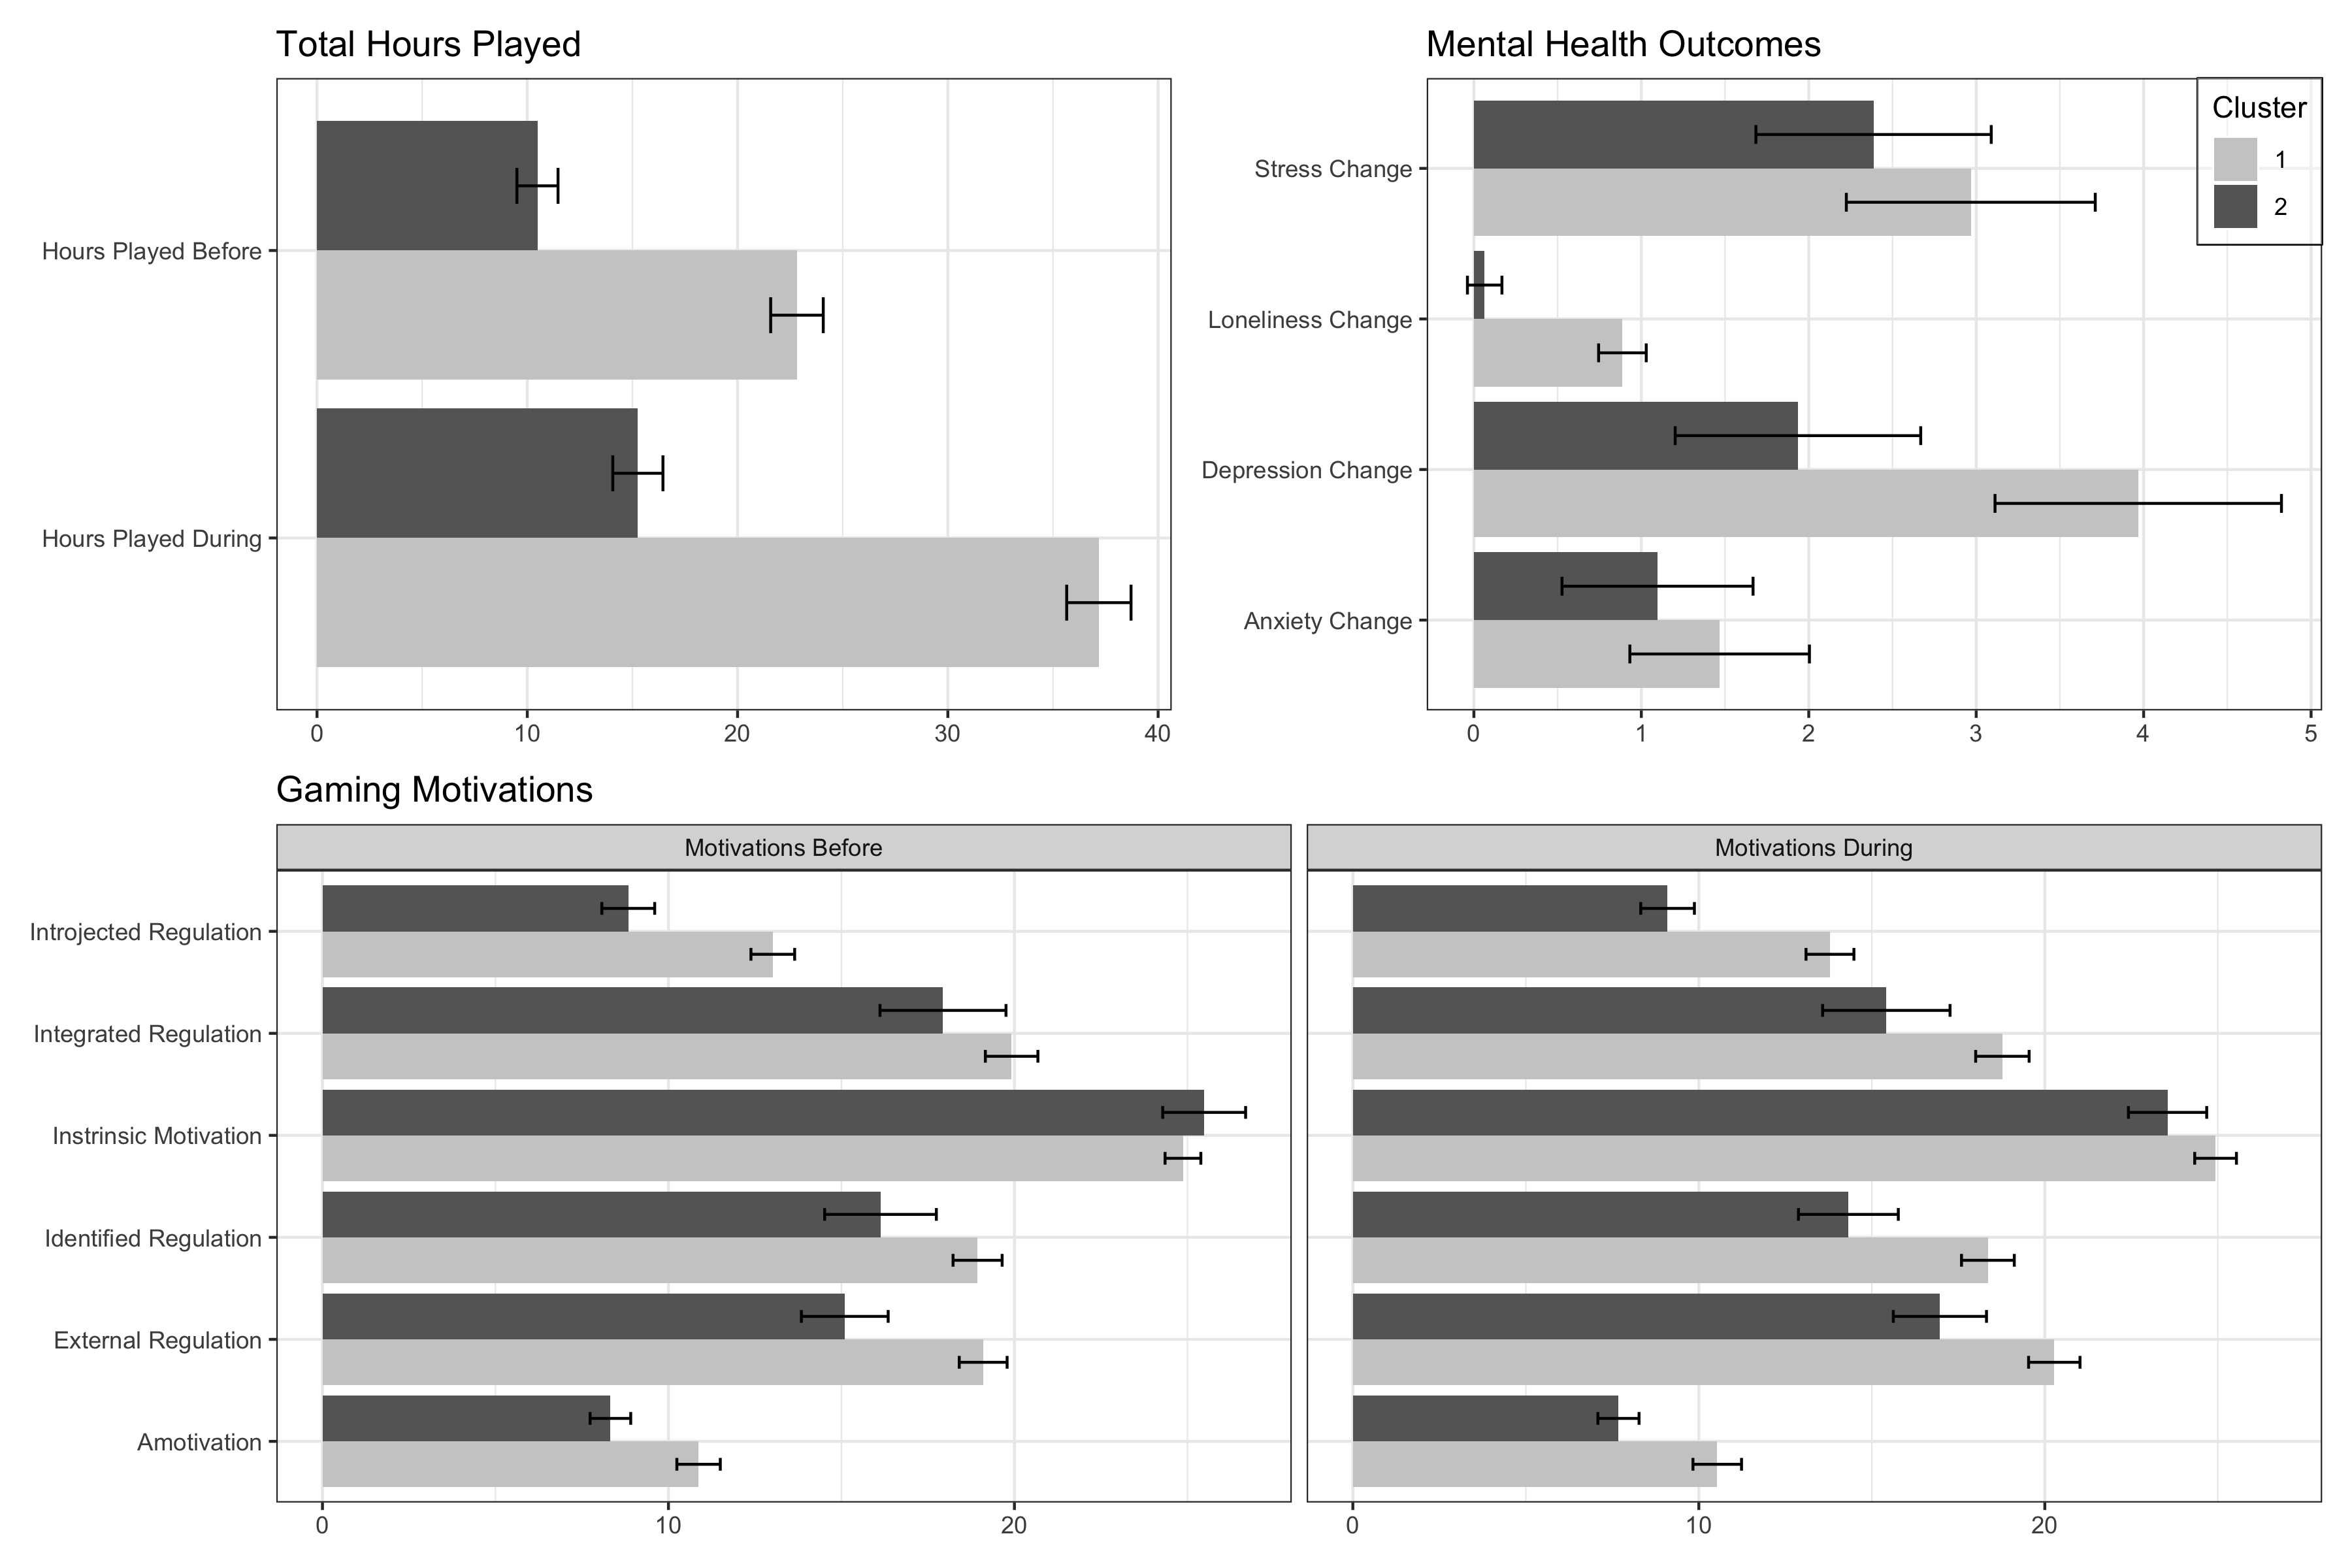
\includegraphics[width=0.9\linewidth]{/Users/glennwilliams/Dropbox/GitHub/covid-gaming/03_plots/cluster_plots} 

}

\caption{ }\label{fig:cluster-plots}
\end{figure*}

Having determined potentially two clusters in the data set, we next evaluated any differences in the hours played and mental health outcomes in the two clusters before conducting a series of correlations between motivations towards gaming and mental health outcomes.

We used the \texttt{BayesFactor} R-package to calculate the Bayes factor for the evidence in support of an difference in hours played beween the two clusters during the time periods before and during lockdown. We again used a default \(Cauchy(0, 0.707)\) prior and estimated the posterior median and 95\% credible intervals using 1000 posterior samples. We found evidence in support of the alternative hypothesis (i.e.~a difference in means) when compared to the null hypothesis (i.e.~no difference in means) for the periods before lockdown, \(BF_{10}\) = 4650.12 (±0\%), \(\Delta{M}\) = 11.53, \(SD\) = 2.68, 95\% CI = {[}6.35, 16.67{]} and after lockdown, \(BF_{10}\) = \textgreater{} 1,000,000 (±0\%), \(\Delta{M}\) = 20.82, \(SD\) = 3.25, 95\% CI = {[}14.38, 27.44{]}. Figure~\ref{fig:cluster-plots} shows that the Cluster 1 spends a larger number of hours per week gaming than Cluster 2. We used the same methods to explore differences between clusters in terms of changes to mental health outcomes. These are summarised in Table~\ref{tab:mh-change-clusts}.

\begin{table*}[tbp]

\begin{center}
\begin{threeparttable}

\caption{\label{tab:mh-change-clusts}Bayes factors for the change in depression, anxiety, stress, and loneliness evaluating evidence in support of the alternative hypothesis (i.e. of a non-null effect)}

\begin{tabular}{lllll}
\toprule
Test & \multicolumn{1}{c}{$\Delta{M}$} & \multicolumn{1}{c}{$SE$} & \multicolumn{1}{c}{95\% CI} & \multicolumn{1}{c}{$BF_{10}$}\\
\midrule
Anxiety Change & 0.31 & 0.03 & [-1.79, 2.35] & 0.22\\
Depression Change & 1.79 & 0.05 & [-1.39, 4.90] & 0.38\\
Stress Change & 0.55 & 0.05 & [-2.22, 3.27] & 0.23\\
Loneliness Change & 0.76 & 0.01 & [0.19, 1.33] & 7.31\\
\bottomrule
\addlinespace
\end{tabular}

\begin{tablenotes}[para]
\normalsize{\textit{Note.} Higher values indicate support for the alternative hypothesis while lower numbers indicate support for the null hypothesis (i.e. of a point-null effect).}
\end{tablenotes}

\end{threeparttable}
\end{center}

\end{table*}

Table~\ref{tab:mh-change-clusts} shows that there is reliable evidence of a difference in the two clusters in terms of changes to loneliness. Observing Figure~\ref{fig:cluster-plots} Cluster 1 shows a greater increase in loneliness as a result of lockdown when compared to Cluster 2.

Finally, we used the same methods to determine any reliable differences in the moitivations for gaming between the two clusters. These are summarised in Table~\ref{tab:motivation-change-clusts}.

\begin{table*}[tbp]

\begin{center}
\begin{threeparttable}

\caption{\label{tab:motivation-change-clusts}Bayes factors for the difference in gaming motivations between the two clusters evaluating evidence in support of the alternative hypothesis (i.e. of a non-null difference)}

\begin{tabular}{lllll}
\toprule
Motivation & \multicolumn{1}{c}{$\Delta{M}$} & \multicolumn{1}{c}{$SE$} & \multicolumn{1}{c}{95\% CI} & \multicolumn{1}{c}{$BF_{10}$}\\
\midrule
Before Lockdown &  &  &  & \\
\ \ \ Amotivation & 2.33 & 0.04 & [-0.13, 4.79] & 1.18\\
\ \ \ External Regulation & 3.58 & 0.05 & [0.59, 6.52] & 4.46\\
\ \ \ Identified Regulation & 2.55 & 0.05 & [-0.51, 5.36] & 0.78\\
\ \ \ Integrated Regulation & 1.69 & 0.05 & [-1.62, 4.77] & 0.37\\
\ \ \ Introjected Regulation & 3.87 & 0.04 & [1.32, 6.20] & 16.82\\
\ \ \ Instrinsic Motivation & -0.49 & 0.03 & [-2.62, 1.60] & 0.24\\
During Lockdown &  &  &  & \\
\ \ \ Amotivation & 2.66 & 0.04 & [-0.10, 5.30] & 1.21\\
\ \ \ External Regulation & 3.03 & 0.05 & [0.15, 6.03] & 1.30\\
\ \ \ Identified Regulation & 3.48 & 0.05 & [0.22, 6.76] & 2.62\\
\ \ \ Integrated Regulation & 3.01 & 0.05 & [-0.15, 6.37] & 0.99\\
\ \ \ Introjected Regulation & 4.27 & 0.04 & [1.71, 6.94] & 22.06\\
\ \ \ Instrinsic Motivation & 1.28 & 0.04 & [-1.06, 3.72] & 0.34\\
\bottomrule
\addlinespace
\end{tabular}

\begin{tablenotes}[para]
\normalsize{\textit{Note.} Higher values indicate support for the alternative hypothesis while lower numbers indicate support for the null hypothesis (i.e. of a point-null difference).}
\end{tablenotes}

\end{threeparttable}
\end{center}

\end{table*}

Table~\ref{tab:motivation-change-clusts} shows that there is reliable evidence of a difference in the two clusters in terms of external regulation and introjected regulation before lockdown and introjected regulation during lockdown. Observing Figure~\ref{fig:cluster-plots} shows that external regulation before lockdown and introjected regulation before and after lockdown is on average larger in Cluster 1 than Cluster 2. Overall, these findings suggest that participants can be clustered such that Cluster 1 has markedly different patterns to Cluster 2 in terms of playing time, loneliness, and motivational factors; Cluster 1 represents gamers who spend a lot of time gaming but who suffer more from loneliness during lockdown and COMMENT ON MOTIVATIONS HERE.

Finally, we performed a series of Bayesian correlations using the same methods outlined above. Posterior means and 95\% credible intervals using 95\% posterior samples. The result of these correlations is shown in Table~\ref{tab:cluster-motivation-correlations}.

\begin{table*}[tbp]

\begin{center}
\begin{threeparttable}

\caption{\label{tab:cluster-motivation-correlations}Correlation coefficients, 95\% credible intervals, and Bayes factors for the correlation between mental health outcomes during lockdown and gaming motivations before and after lockdown for each cluster.}

\begin{tabular}{lllll}
\toprule
Outcome & \multicolumn{1}{c}{Amotivation Before} & \multicolumn{1}{c}{Amotivation After} & \multicolumn{1}{c}{Instrinsic Motivation Before} & \multicolumn{1}{c}{Instrinsic Motivation After}\\
\midrule
Cluster One &  &  &  & \\
\ \ \ Depression After & \makecell[c]{0.29 [0.13, 0.44], \\$BF_{10}$ = 57.59} & \makecell[c]{0.35 [0.19, 0.5], \\$BF_{10}$ = 1307.26} & \makecell[c]{0.07 [-0.11, 0.23], \\$BF_{10}$ = 0.27} & \makecell[c]{0.1 [-0.06, 0.26], \\$BF_{10}$ = 0.42}\\
\ \ \ Stress After & \makecell[c]{0.31 [0.13, 0.46], \\$BF_{10}$ = 121.95} & \makecell[c]{0.25 [0.08, 0.41], \\$BF_{10}$ = 14.72} & \makecell[c]{0.21 [0.04, 0.36], \\$BF_{10}$ = 4.08} & \makecell[c]{0.26 [0.1, 0.41], \\$BF_{10}$ = 19.54}\\
\ \ \ Anxiety After & \makecell[c]{0.22 [0.05, 0.37], \\$BF_{10}$ = 5.07} & \makecell[c]{0.21 [0.05, 0.37], \\$BF_{10}$ = 3.86} & \makecell[c]{0.19 [0.03, 0.35], \\$BF_{10}$ = 2.22} & \makecell[c]{0.23 [0.05, 0.39], \\$BF_{10}$ = 6.04}\\
\ \ \ Loneliness After & \makecell[c]{0.16 [-0.01, 0.33], \\$BF_{10}$ = 1.19} & \makecell[c]{0.28 [0.11, 0.43], \\$BF_{10}$ = 33.83} & \makecell[c]{-0.07 [-0.24, 0.1], \\$BF_{10}$ = 0.27} & \makecell[c]{0.09 [-0.07, 0.25], \\$BF_{10}$ = 0.37}\\
Cluster Two &  &  &  & \\
\ \ \ Depression After & \makecell[c]{0.07 [-0.24, 0.38], \\$BF_{10}$ = 0.42} & \makecell[c]{0.25 [-0.04, 0.52], \\$BF_{10}$ = 1.26} & \makecell[c]{0.15 [-0.17, 0.46], \\$BF_{10}$ = 0.59} & \makecell[c]{0.09 [-0.23, 0.4], \\$BF_{10}$ = 0.46}\\
\ \ \ Stress After & \makecell[c]{0.03 [-0.29, 0.36], \\$BF_{10}$ = 0.40} & \makecell[c]{0.2 [-0.1, 0.5], \\$BF_{10}$ = 0.86} & \makecell[c]{0.19 [-0.14, 0.47], \\$BF_{10}$ = 0.75} & \makecell[c]{0.14 [-0.19, 0.44], \\$BF_{10}$ = 0.58}\\
\ \ \ Anxiety After & \makecell[c]{0 [-0.31, 0.32], \\$BF_{10}$ = 0.39} & \makecell[c]{0.18 [-0.13, 0.47], \\$BF_{10}$ = 0.69} & \makecell[c]{0.09 [-0.23, 0.41], \\$BF_{10}$ = 0.46} & \makecell[c]{0.04 [-0.25, 0.36], \\$BF_{10}$ = 0.41}\\
\ \ \ Loneliness After & \makecell[c]{0.16 [-0.17, 0.46], \\$BF_{10}$ = 0.64} & \makecell[c]{0.04 [-0.28, 0.36], \\$BF_{10}$ = 0.41} & \makecell[c]{-0.08 [-0.4, 0.25], \\$BF_{10}$ = 0.43} & \makecell[c]{-0.01 [-0.31, 0.32], \\$BF_{10}$ = 0.39}\\
\bottomrule
\addlinespace
\end{tabular}

\begin{tablenotes}[para]
\normalsize{\textit{Note.} Higher values indicate support for the alternative hypothesis while lower numbers indicate support for the null hypothesis (i.e. of a point-null effect).}
\end{tablenotes}

\end{threeparttable}
\end{center}

\end{table*}

In Cluster 1, there is a positive correlation between amotivation before lockdown and all mental health outcomes excluding loneliness. There is also a positive correlation between amotivation after lockdown and all mental health outcomes. Thus, a lack of motivation for gaming likely reflects poor mental health outcomes. Here, there is a also negative correlation between intrinsic motivation before lockdown and depression and loneliness after lockdown. This indicates that a motivation to play games is associated with better depression and loneliness scores. However, there is a weak positive correlation between intrinstic motivation before lockdown and stress after lockdown. IM UNSURE WHAT THIS COULD MEAN. Additionally, there is a positive correlation between intrinsic motivation after lockdown both stress and anxiety after lockdown. IM UNSURE WHAT THIS COULD MEAN. -- PERHAPS PEOPLE WHO WANT TO GAME CAN'T BECAUSE THEY HAVE TO WORK?

In Cluster 2, there is no evidence for a reliable correlation between any of the motivational factors of gaming and mental health outcomes. Here, the Bayes factors all show weak evidence in one direction or another, indicating insensitivity of the tests to properly evaluate the hypotheses.

\hypertarget{moderation-analyses}{%
\subsection{Moderation analyses}\label{moderation-analyses}}

Finally, we explored whether the effect of motivation on mental health outcomes is moderated by loneliness.

Models used\ldots DETAILS ON PRIORS NEEDED.

We present posterior predictions for the effect of difference in hours played pre- and post-lockdown on differences in outcomes for each subscale. Here, lines represent the posterior median along with 95\% credible intervals (shaded).

We found no evidence of moderation for depression, stress, or anxiety as a function of loneliness and amotivation during lockdown.

\begin{figure*}[!htbp]

{\centering 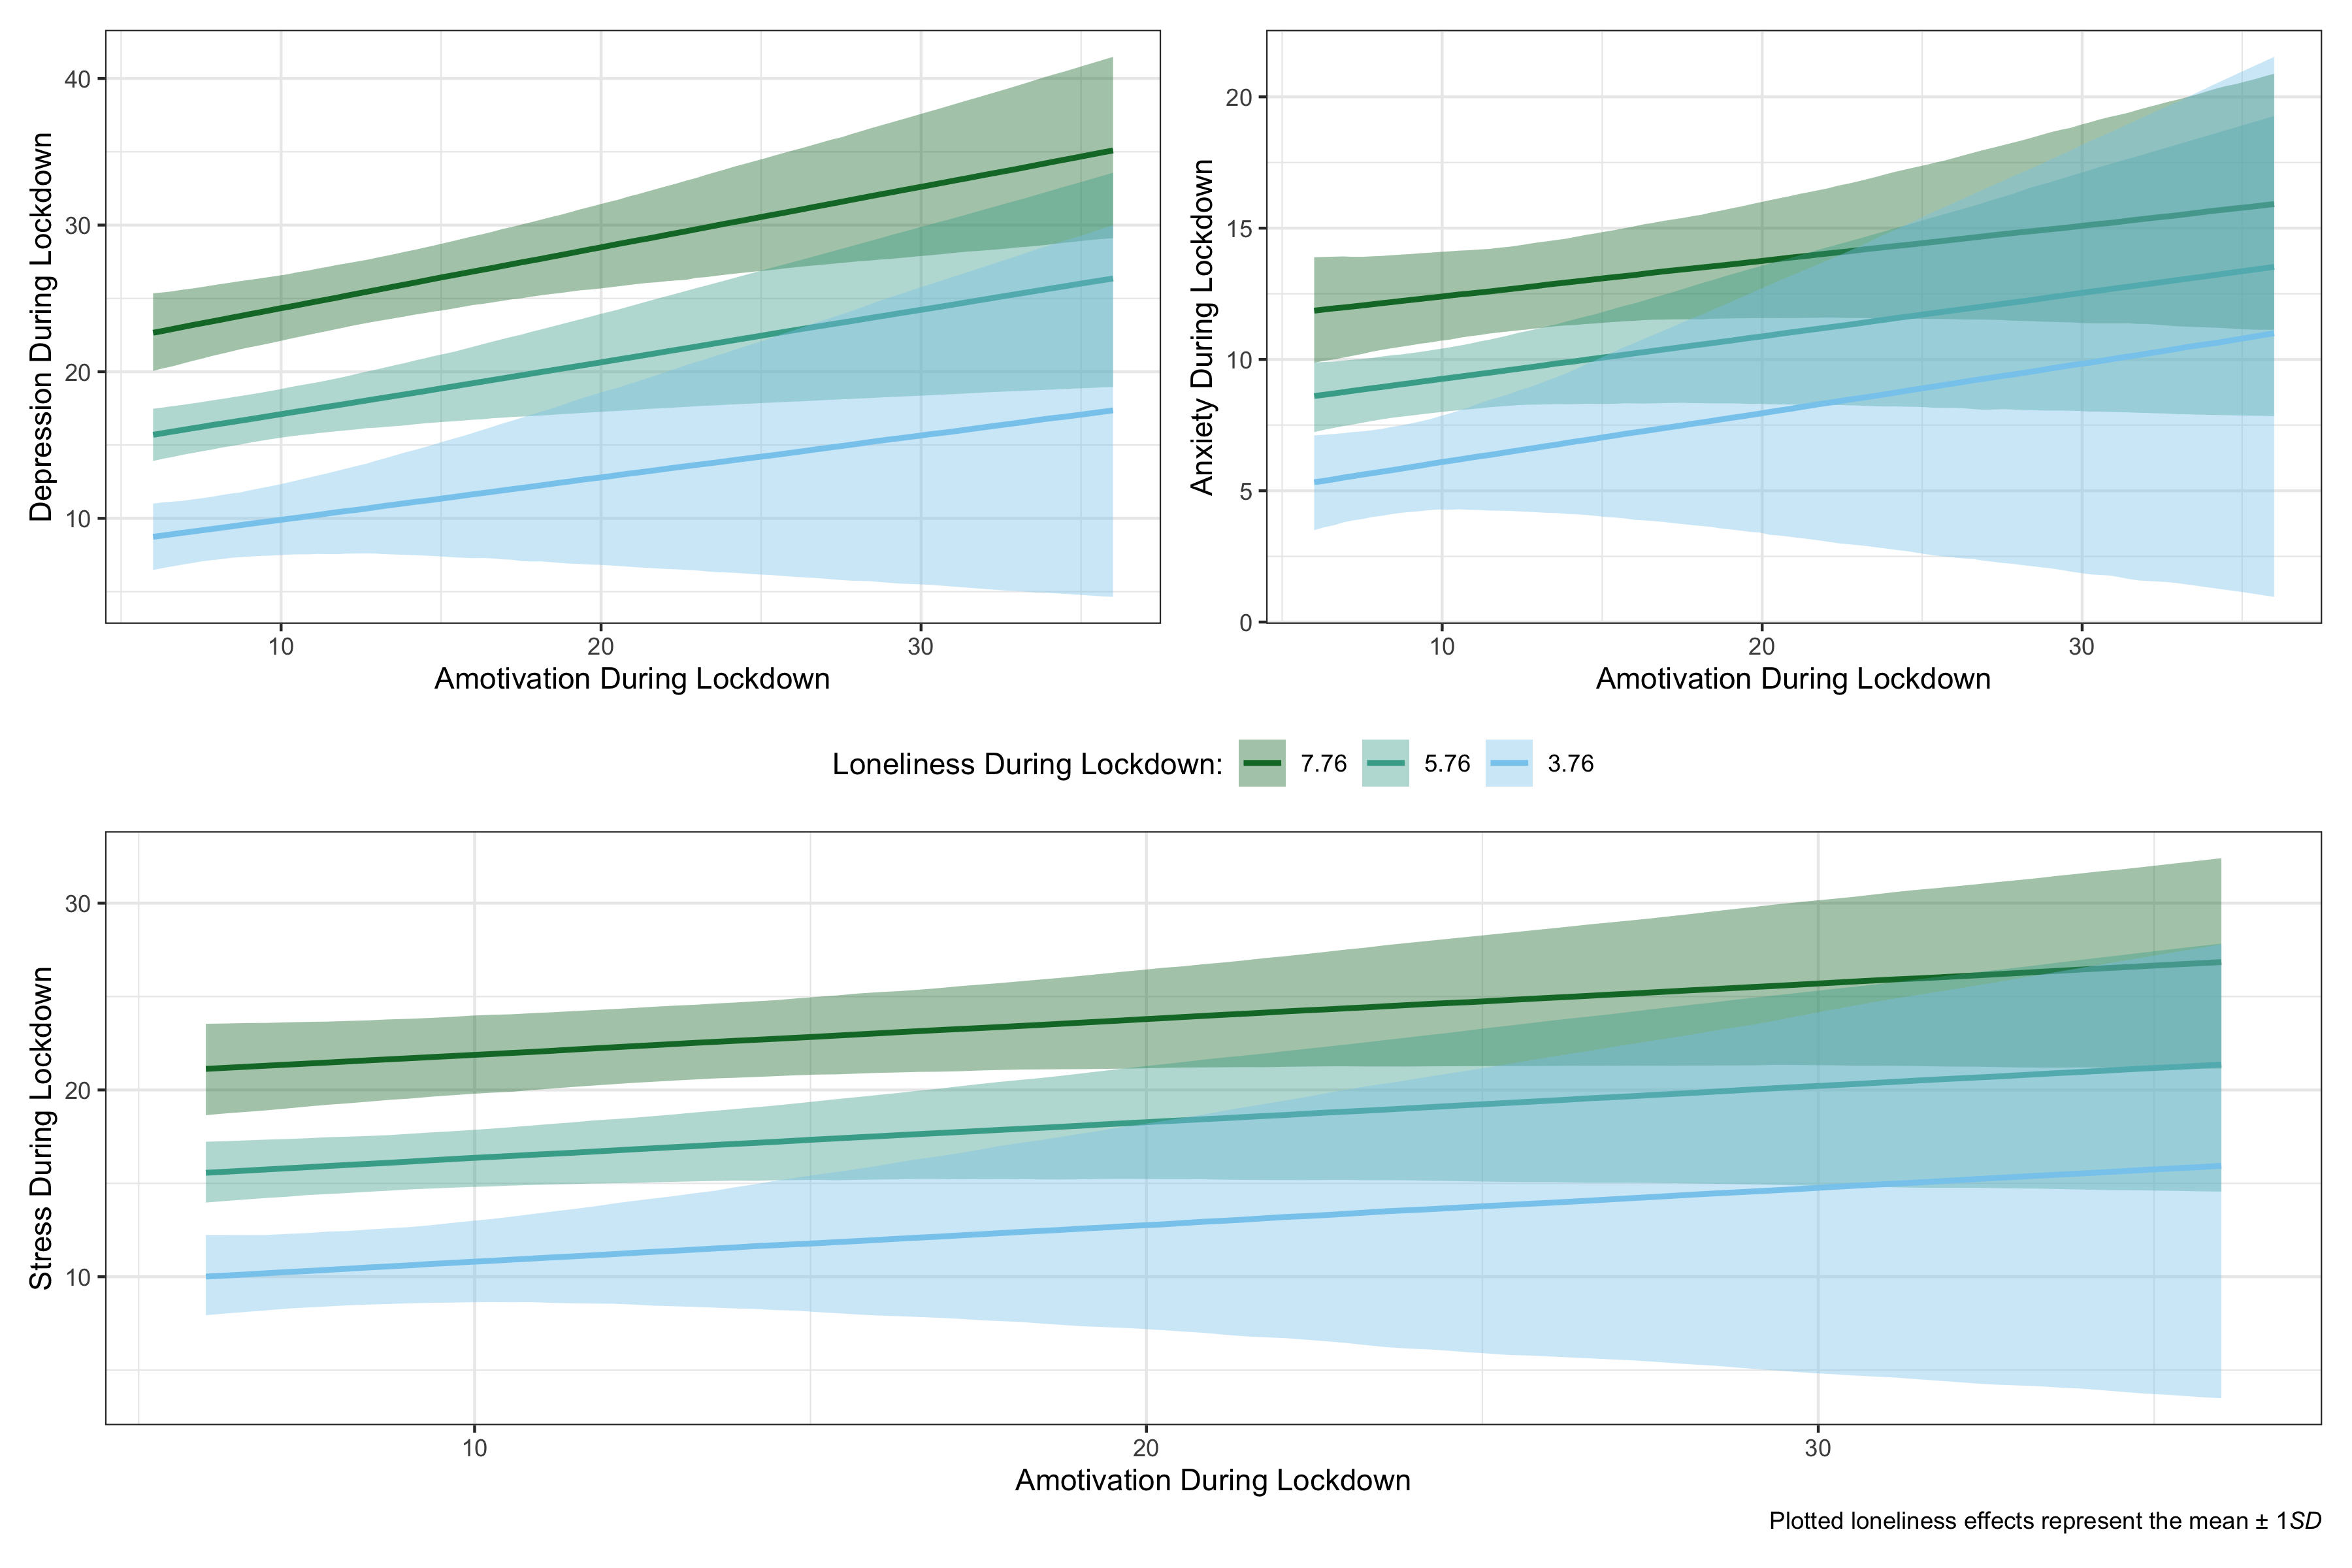
\includegraphics[width=0.9\linewidth]{/Users/glennwilliams/Dropbox/GitHub/covid-gaming/03_plots/amotivation_moderation_plot} 

}

\caption{ }\label{fig:amotivation-moderation-plot}
\end{figure*}

Similarly, we found no reliable evidence of moderation for depression, anxiety, and stress as a function of loneliness and intrinsic motivation during lockdown.

\begin{figure*}[!htbp]

{\centering 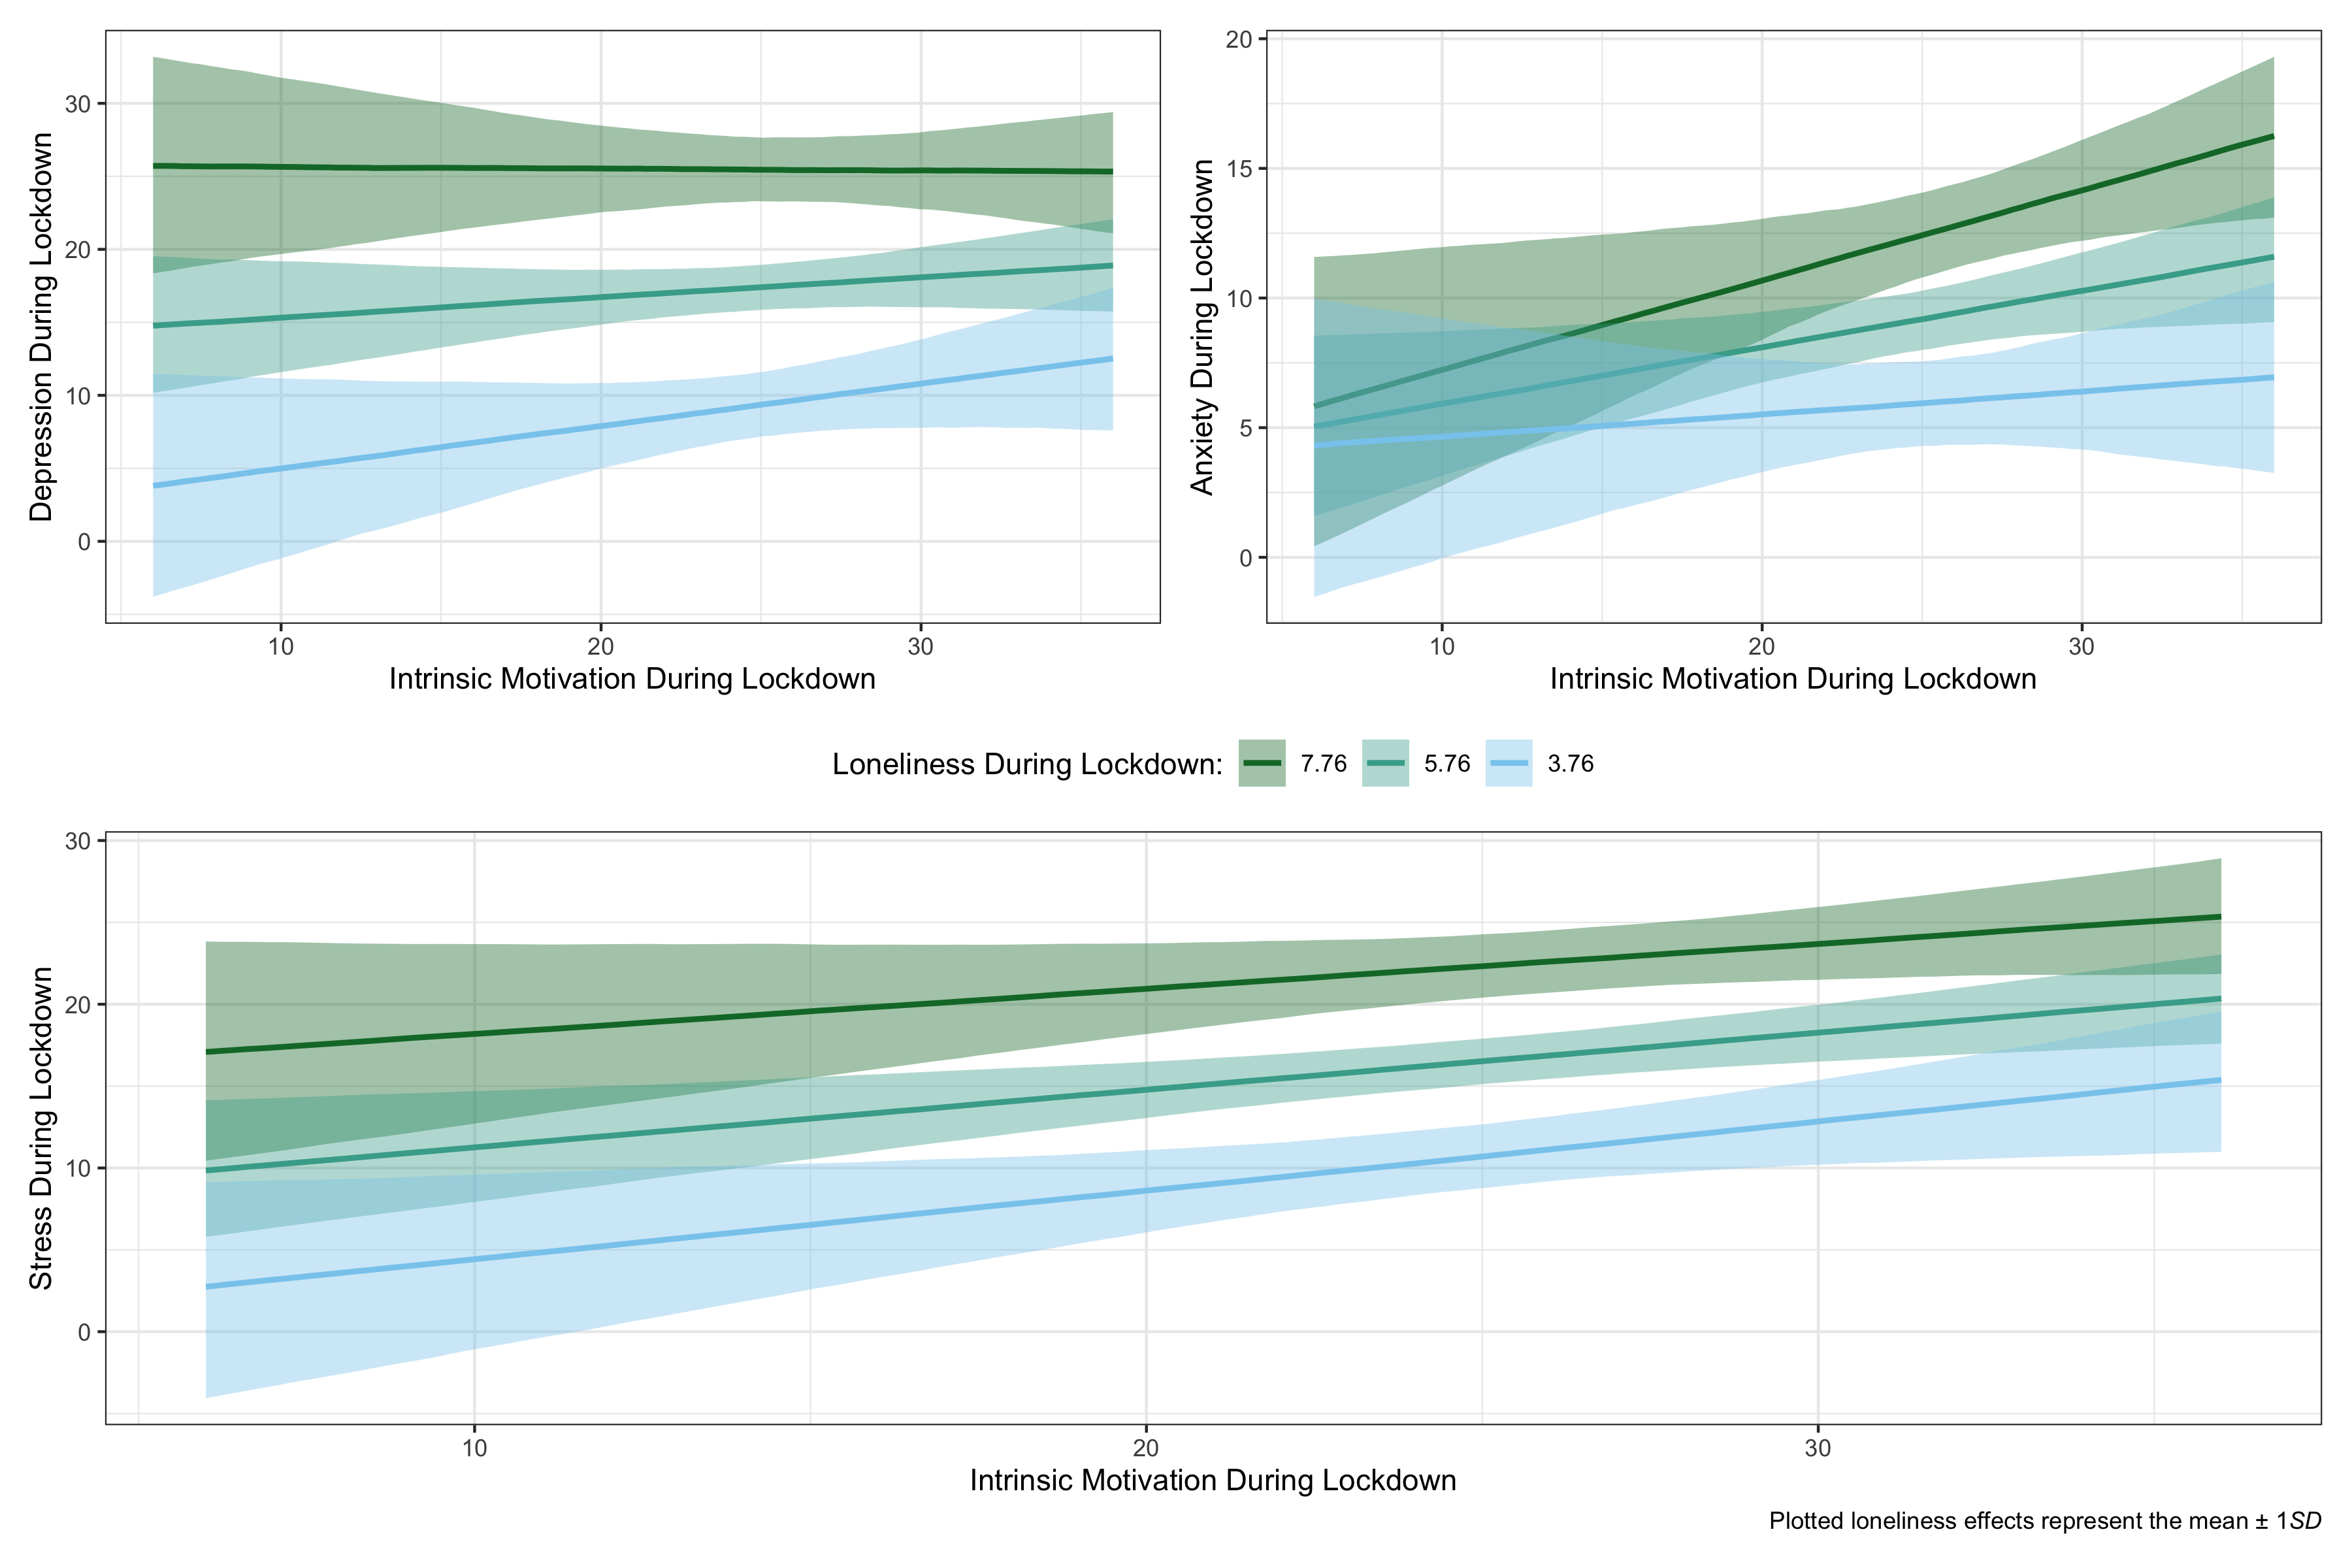
\includegraphics[width=0.9\linewidth]{/Users/glennwilliams/Dropbox/GitHub/covid-gaming/03_plots/intrinsic_moderation_plot} 

}

\caption{ }\label{fig:intrinsic-moderation-plot}
\end{figure*}

Question: Do we need this for the clusters too? This is already far too much for one study\ldots{}

\hypertarget{discussion}{%
\section{Discussion}\label{discussion}}

Discussion here.

\newpage

\hypertarget{references}{%
\section{References}\label{references}}

\begingroup
\setlength{\parindent}{-0.5in}
\setlength{\leftskip}{0.5in}

\hypertarget{refs}{}
\leavevmode\hypertarget{ref-R-papaja}{}%
Aust, F., \& Barth, M. (2020). \emph{papaja: Create APA manuscripts with R Markdown}. Retrieved from \url{https://github.com/crsh/papaja}

\leavevmode\hypertarget{ref-R-Matrix}{}%
Bates, D., \& Maechler, M. (2019). \emph{Matrix: Sparse and dense matrix classes and methods}. Retrieved from \url{https://CRAN.R-project.org/package=Matrix}

\leavevmode\hypertarget{ref-R-brms_a}{}%
Bürkner, P.-C. (2017). brms: An R package for Bayesian multilevel models using Stan. \emph{Journal of Statistical Software}, \emph{80}(1), 1--28. \url{https://doi.org/10.18637/jss.v080.i01}

\leavevmode\hypertarget{ref-R-brms_b}{}%
Bürkner, P.-C. (2018). Advanced Bayesian multilevel modeling with the R package brms. \emph{The R Journal}, \emph{10}(1), 395--411. \url{https://doi.org/10.32614/RJ-2018-017}

\leavevmode\hypertarget{ref-R-Rcpp_b}{}%
Eddelbuettel, D., \& Balamuta, J. J. (2017). Extending extitR with extitC++: A Brief Introduction to extitRcpp. \emph{PeerJ Preprints}, \emph{5}, e3188v1. \url{https://doi.org/10.7287/peerj.preprints.3188v1}

\leavevmode\hypertarget{ref-R-Rcpp_a}{}%
Eddelbuettel, D., \& François, R. (2011). Rcpp: Seamless R and C++ integration. \emph{Journal of Statistical Software}, \emph{40}(8), 1--18. \url{https://doi.org/10.18637/jss.v040.i08}

\leavevmode\hypertarget{ref-R-janitor}{}%
Firke, S. (2020). \emph{Janitor: Simple tools for examining and cleaning dirty data}. Retrieved from \url{https://CRAN.R-project.org/package=janitor}

\leavevmode\hypertarget{ref-R-english}{}%
Fox, J., Venables, B., Damico, A., \& Salverda, A. P. (2020). \emph{English: Translate integers into english}. Retrieved from \url{https://CRAN.R-project.org/package=english}

\leavevmode\hypertarget{ref-R-flextable}{}%
Gohel, D. (2021). \emph{Flextable: Functions for tabular reporting}. Retrieved from \url{https://CRAN.R-project.org/package=flextable}

\leavevmode\hypertarget{ref-R-lubridate}{}%
Grolemund, G., \& Wickham, H. (2011). Dates and times made easy with lubridate. \emph{Journal of Statistical Software}, \emph{40}(3), 1--25. Retrieved from \url{http://www.jstatsoft.org/v40/i03/}

\leavevmode\hypertarget{ref-R-purrr}{}%
Henry, L., \& Wickham, H. (2020). \emph{Purrr: Functional programming tools}. Retrieved from \url{https://CRAN.R-project.org/package=purrr}

\leavevmode\hypertarget{ref-R-factoextra}{}%
Kassambara, A., \& Mundt, F. (2020). \emph{Factoextra: Extract and visualize the results of multivariate data analyses}. Retrieved from \url{https://CRAN.R-project.org/package=factoextra}

\leavevmode\hypertarget{ref-R-tidybayes}{}%
Kay, M. (2020). \emph{tidybayes: Tidy data and geoms for Bayesian models}. \url{https://doi.org/10.5281/zenodo.1308151}

\leavevmode\hypertarget{ref-R-interactions}{}%
Long, J. A. (2019). \emph{Interactions: Comprehensive, user-friendly toolkit for probing interactions}. Retrieved from \url{https://cran.r-project.org/package=interactions}

\leavevmode\hypertarget{ref-R-BayesFactor}{}%
Morey, R. D., \& Rouder, J. N. (2018). \emph{BayesFactor: Computation of bayes factors for common designs}. Retrieved from \url{https://CRAN.R-project.org/package=BayesFactor}

\leavevmode\hypertarget{ref-R-here}{}%
Müller, K. (2017). \emph{Here: A simpler way to find your files}. Retrieved from \url{https://CRAN.R-project.org/package=here}

\leavevmode\hypertarget{ref-R-tibble}{}%
Müller, K., \& Wickham, H. (2020). \emph{Tibble: Simple data frames}. Retrieved from \url{https://CRAN.R-project.org/package=tibble}

\leavevmode\hypertarget{ref-R-patchwork}{}%
Pedersen, T. L. (2020). \emph{Patchwork: The composer of plots}. Retrieved from \url{https://CRAN.R-project.org/package=patchwork}

\leavevmode\hypertarget{ref-R-ggforce}{}%
Pedersen, T. L. (2021). \emph{Ggforce: Accelerating 'ggplot2'}. Retrieved from \url{https://CRAN.R-project.org/package=ggforce}

\leavevmode\hypertarget{ref-R-raincloudplots}{}%
person). (2021). \emph{Raincloudplots: The easy way to create raincloud plots}. Retrieved from \url{https://github.com/jorvlan/raincloudplots}

\leavevmode\hypertarget{ref-R-coda}{}%
Plummer, M., Best, N., Cowles, K., \& Vines, K. (2006). CODA: Convergence diagnosis and output analysis for mcmc. \emph{R News}, \emph{6}(1), 7--11. Retrieved from \url{https://journal.r-project.org/archive/}

\leavevmode\hypertarget{ref-R-base}{}%
R Core Team. (2020). \emph{R: A language and environment for statistical computing}. Vienna, Austria: R Foundation for Statistical Computing. Retrieved from \url{https://www.R-project.org/}

\leavevmode\hypertarget{ref-R-psych}{}%
Revelle, W. (2020). \emph{Psych: Procedures for psychological, psychometric, and personality research}. Evanston, Illinois: Northwestern University. Retrieved from \url{https://CRAN.R-project.org/package=psych}

\leavevmode\hypertarget{ref-R-mclust}{}%
Scrucca, L., Fop, M., Murphy, T. B., \& Raftery, A. E. (2016). mclust 5: Clustering, classification and density estimation using Gaussian finite mixture models. \emph{The R Journal}, \emph{8}(1), 289--317. Retrieved from \url{https://doi.org/10.32614/RJ-2016-021}

\leavevmode\hypertarget{ref-R-ggplot2}{}%
Wickham, H. (2016). \emph{Ggplot2: Elegant graphics for data analysis}. Springer-Verlag New York. Retrieved from \url{https://ggplot2.tidyverse.org}

\leavevmode\hypertarget{ref-R-stringr}{}%
Wickham, H. (2019). \emph{Stringr: Simple, consistent wrappers for common string operations}. Retrieved from \url{https://CRAN.R-project.org/package=stringr}

\leavevmode\hypertarget{ref-R-forcats}{}%
Wickham, H. (2020a). \emph{Forcats: Tools for working with categorical variables (factors)}. Retrieved from \url{https://CRAN.R-project.org/package=forcats}

\leavevmode\hypertarget{ref-R-modelr}{}%
Wickham, H. (2020b). \emph{Modelr: Modelling functions that work with the pipe}. Retrieved from \url{https://CRAN.R-project.org/package=modelr}

\leavevmode\hypertarget{ref-R-tidyr}{}%
Wickham, H. (2020c). \emph{Tidyr: Tidy messy data}. Retrieved from \url{https://CRAN.R-project.org/package=tidyr}

\leavevmode\hypertarget{ref-R-tidyverse}{}%
Wickham, H., Averick, M., Bryan, J., Chang, W., McGowan, L. D., François, R., \ldots{} Yutani, H. (2019). Welcome to the tidyverse. \emph{Journal of Open Source Software}, \emph{4}(43), 1686. \url{https://doi.org/10.21105/joss.01686}

\leavevmode\hypertarget{ref-R-dplyr}{}%
Wickham, H., François, R., Henry, L., \& Müller, K. (2020). \emph{Dplyr: A grammar of data manipulation}. Retrieved from \url{https://CRAN.R-project.org/package=dplyr}

\leavevmode\hypertarget{ref-R-readr}{}%
Wickham, H., Hester, J., \& Francois, R. (2018). \emph{Readr: Read rectangular text data}. Retrieved from \url{https://CRAN.R-project.org/package=readr}

\leavevmode\hypertarget{ref-R-kableExtra}{}%
Zhu, H. (2020). \emph{KableExtra: Construct complex table with 'kable' and pipe syntax}. Retrieved from \url{https://CRAN.R-project.org/package=kableExtra}

\endgroup


\end{document}
